%!TEX root = ../dissertation.tex
\begin{savequote}[75mm]
A fruit must rot before its seed can sprout.   
\end{savequote}
\chapter{Validations with low mass and high mass signal region}
\label{app:appendixZZ}

\paragraph{}
Another check is the the so-called ``low mass signal region'' (or ZZ region) and ``high mass signal region'' (or TT region). 
On the \mleadJ-\msublJ~ 2D plane, a lower in center (ZZ) and higher in center (TT) signal region are defined: 
\begin{equation}
X_{ZZ} = \sqrt{\left(\frac{m^{\rm lead}_{\rm J} - \text{103 GeV}}{0.1 \left(m^{\rm lead}_{\rm J}\right)}\right)^2 + \left(\frac{m^{\rm subl}_{\rm J}- \text{96 GeV}}{0.1 \left(m^{\rm subl}_{\rm J}\right)}\right)^2}
\label{eq:boosted_Xzz}
\end{equation}
\begin{equation}
X_{TT} = \sqrt{\left(\frac{m^{\rm lead}_{\rm J} - \text{164 GeV}}{0.1 \left(m^{\rm lead}_{\rm J}\right)}\right)^2 + \left(\frac{m^{\rm subl}_{\rm J}- \text{155 GeV}}{0.1 \left(m^{\rm subl}_{\rm J}\right)}\right)^2}
\label{eq:boosted_Xtt}
\end{equation}
They are shown in Figure~\ref{fig:ZZIllustration}. 
The signal region background is estimated using the same sideband and control regions with events contained in the ZZ or TT signal region excluded. 
Then these fake signal regions are unblinded and compared with the prediction. 
This comparison validates the background estimation strategy in QCD and \ttbar~ enriched regions.

\begin{figure}[htb!]
\begin{center}
\captionsetup{justification=centering}
    \begin{subfigure}[b]{0.45\textwidth}
        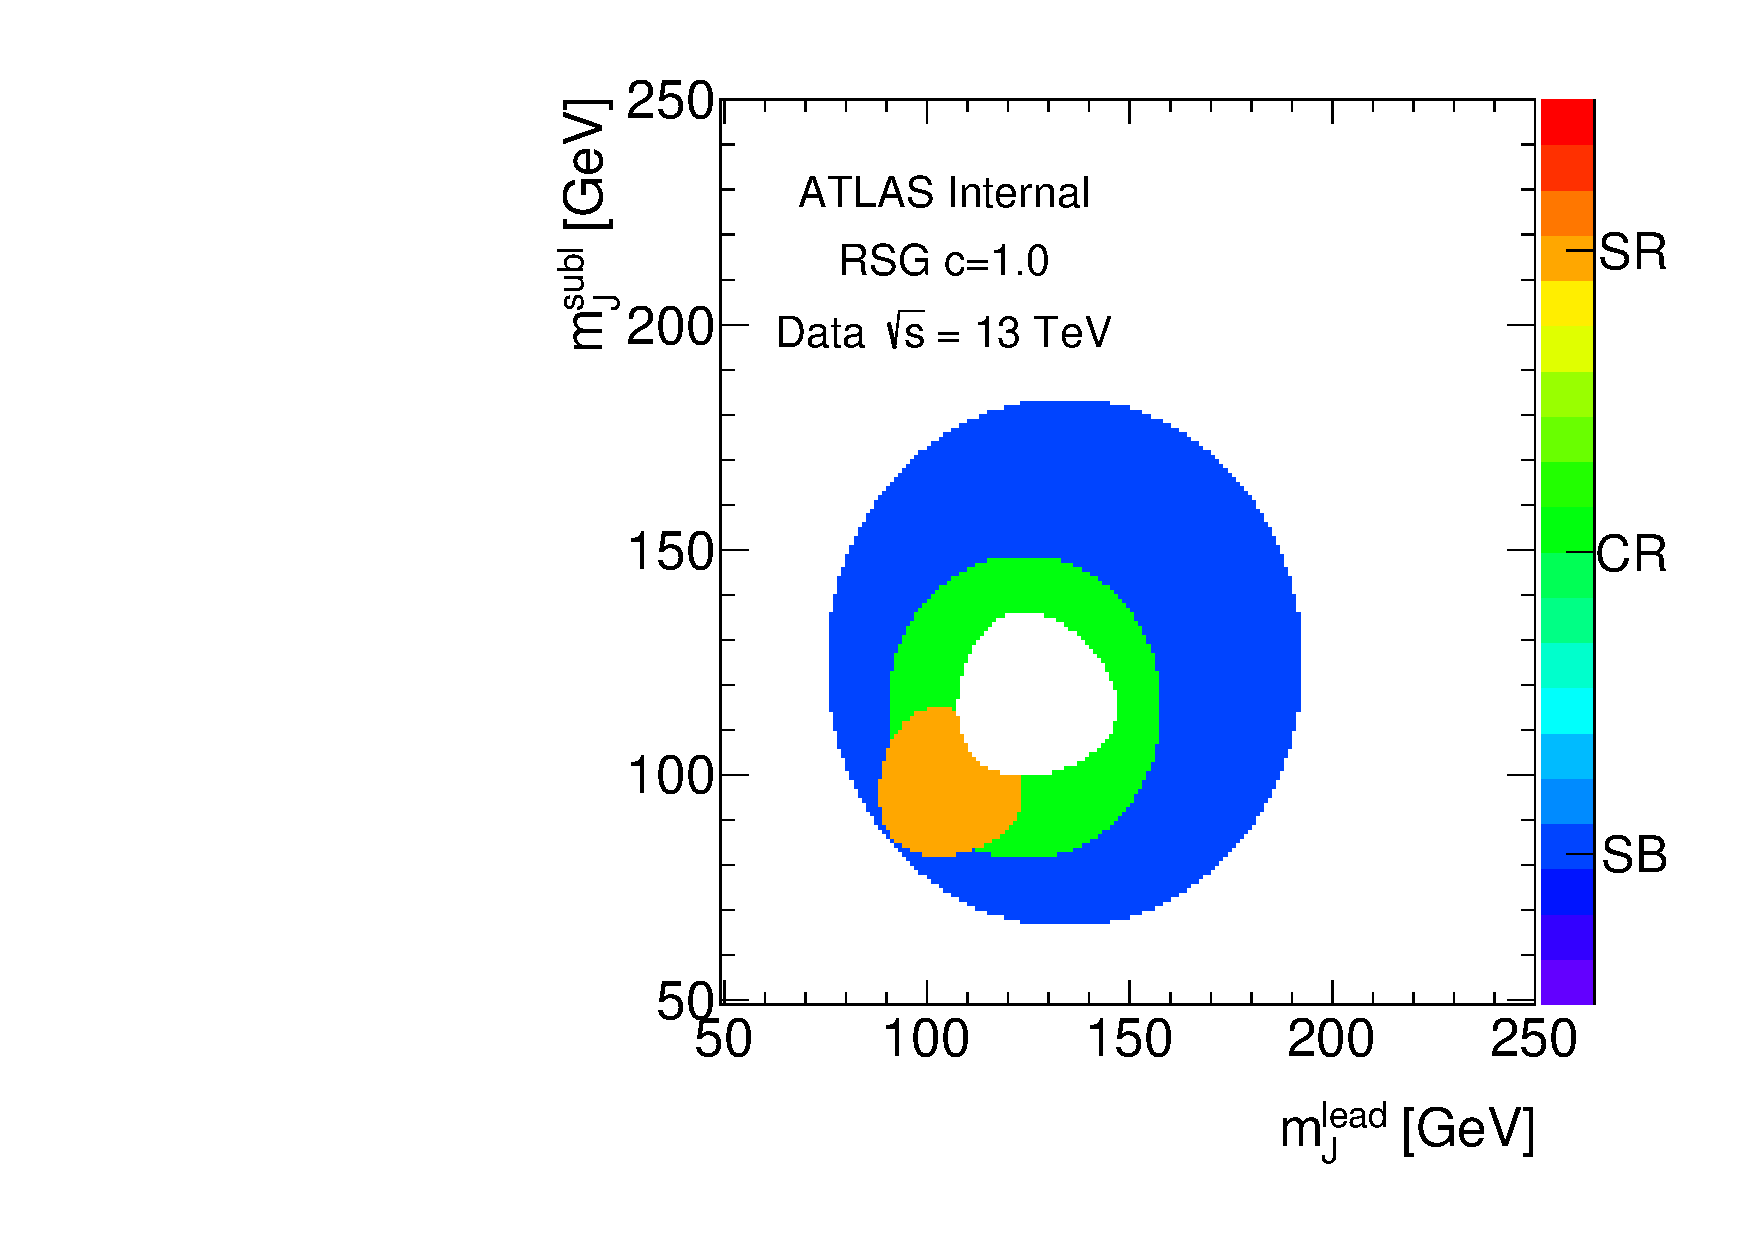
\includegraphics[width=\textwidth,angle=-90]{figures/boosted/ZZ/Compare_NoTag_mH0H1.pdf}
        \caption{ZZ}
        \label{fig:ZZIllustration-ZZ}
    \end{subfigure}
    \quad 
    \begin{subfigure}[b]{0.45\textwidth}
        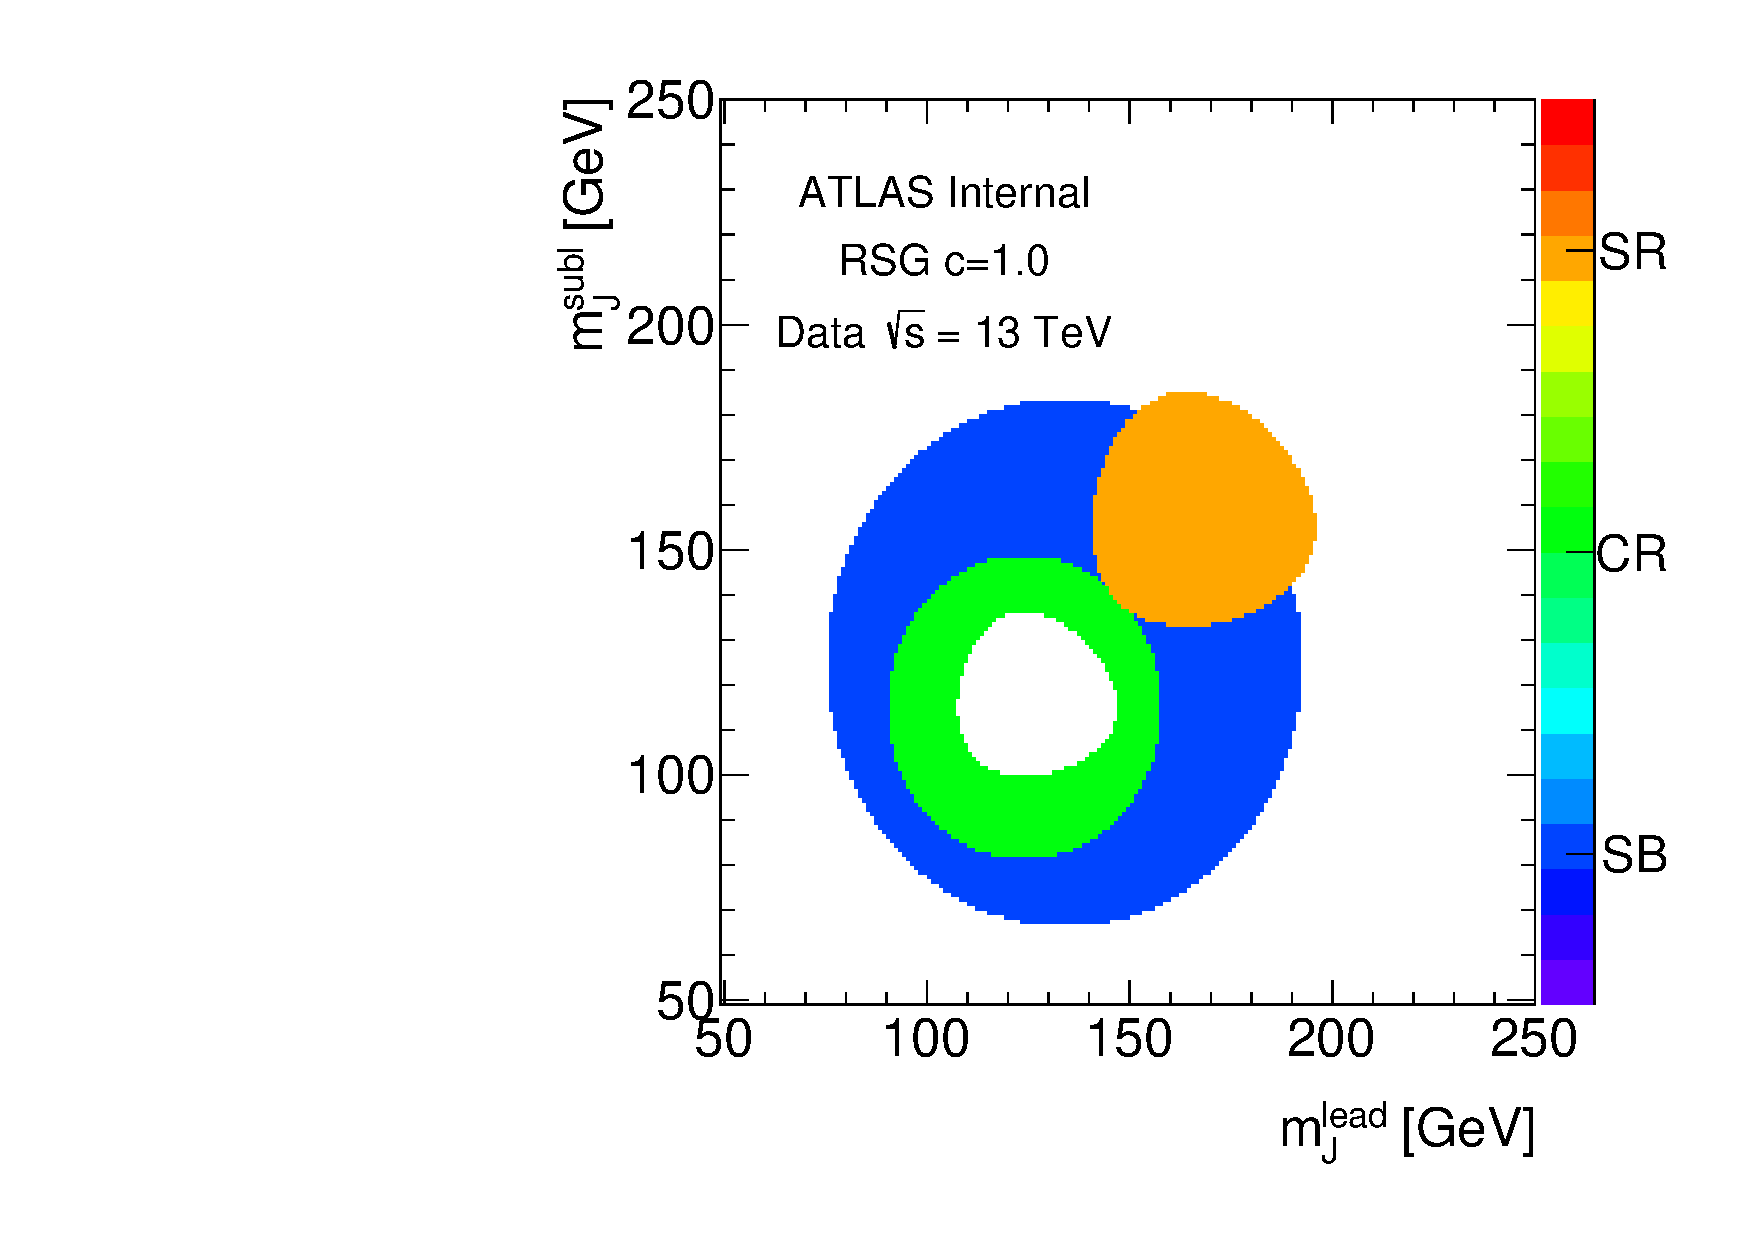
\includegraphics[width=\textwidth,angle=-90]{figures/boosted/TT/Compare_NoTag_mH0H1.pdf}
        \caption{TT}
        \label{fig:ZZIllustration-TT}
    \end{subfigure}
\end{center}
\caption{Illustration of ZZ and TT signal regions on the 2D \mleadJ-\msublJ~ plane. The white circle in the middle is the blinded real signal region.}
\label{fig:ZZIllustration}
\end{figure}

\paragraph{}
%The summary of background estimation for ZZ signal region can be found in Table \ref{CRSB:SummaryTable_ZZ_4b}, ~\ref{CRSB:SummaryTable_ZZ_3b} and ~\ref{CRSB:SummaryTable_ZZ_2b}. 
The differences between data and prediction in the ZZ and TT signal regions are summarized in Tables~\ref{tab:DataPred_zzSR} and \ref{tab:DataPred_ttSR}. 
The kinematic distribution of data and prediction in the ZZ and TT signal regions are shown in Figures~\ref{fig:ZZSR_Distribution} and ~\ref{fig:TTSR_Distribution}.
The differences between data and prediction are comparable with data statistical uncertainties. 

% \begin{table}[htb!]
% \begin{center}
% \begin{footnotesize} 
\begin{tabular}{c|c|c|c} 
FourTag & Sideband & Control & Signal \\ 
\hline\hline 
QCD Est & 166.65 $\pm$ 2.88 & 45.83 $\pm$ 1.51 & 27.37 $\pm$ 1.16\\ 
$t\bar{t}$ Est.  & 27.52 $\pm$ 0.25 & 6.31 $\pm$ 0.14 & 0 $\pm$ 0\\ 
$Z+jets$ & 0 $\pm$ 0 & 6.18 $\pm$ 5.12 & 0 $\pm$ 0\\ 
Total Bkg Est & 194.17 $\pm$ 2.89 & 58.32 $\pm$ 5.34 & 27.37 $\pm$ 1.16\\ 
Data & 194.0 $\pm$ 13.93 & 54.0 $\pm$ 7.35 & 37.0 $\pm$ 6.08\\ 
$c=1.0$,$m=1.0TeV$ & 2.45 $\pm$ 0.098 & 4.47 $\pm$ 0.13 & 0.99 $\pm$ 0.063\\ 
$c=1.0$,$m=2.0TeV$ & 0.032 $\pm$ 0.0015 & 0.075 $\pm$ 0.0022 & 0.028 $\pm$ 0.0014\\ 
$c=1.0$,$m=3.0TeV$ & 0.00029 $\pm$ 3.5e-05 & 0.00064 $\pm$ 5e-05 & 0.0002 $\pm$ 2.7e-05\\ 
\hline\hline 
\end{tabular} 
\end{footnotesize} 
\newline 

% \end{center}
% \caption{Background prediction in SR/CR/SB for ZZ SR in $4b$-tag region. Uncertainties are stat only.}
% \label{CRSB:SummaryTable_ZZ_4b}
% \end{table}

% \begin{table}[htb!]
% \begin{center}
% \begin{footnotesize} 
\begin{tabular}{c|c|c|c} 
ThreeTag & Sideband & Control & Signal \\ 
\hline\hline 
& & & \\ 
QCD Est & 3344.46 $\pm$ 26.85 & 998.41 $\pm$ 14.63 & 637.78 $\pm$ 11.87\\ 
$t\bar{t}$ Est.  & 826.66 $\pm$ 25.11 & 136.58 $\pm$ 10.23 & 30.07 $\pm$ 1.24\\ 
$Z+jets$ & 32.49 $\pm$ 11.34 & 8.22 $\pm$ 5.29 & 3.3 $\pm$ 2.0\\ 
Total Bkg Est & 4203.61 $\pm$ 38.47 & 1143.2 $\pm$ 18.62 & 671.15 $\pm$ 12.11\\ 
Data & 4203.0 $\pm$ 64.83 & 1108.0 $\pm$ 33.29 & 645.0 $\pm$ 25.4\\ 
$c=1.0$,$m=1.0TeV$ & 7.56 $\pm$ 0.18 & 9.84 $\pm$ 0.2 & 3.05 $\pm$ 0.11\\ 
$c=1.0$,$m=2.0TeV$ & 0.15 $\pm$ 0.0033 & 0.27 $\pm$ 0.0046 & 0.12 $\pm$ 0.003\\ 
$c=1.0$,$m=3.0TeV$ & 0.0034 $\pm$ 0.00012 & 0.0056 $\pm$ 0.00016 & 0.0021 $\pm$ 9.5e-05\\ 
& & & \\ 
\hline\hline 
\end{tabular} 
\end{footnotesize} 
\newline 

% \end{center}
% \caption{Background prediction in SR/CR/SB for ZZ SR in $3b$-tag region. Uncertainties are stat only.}
% \label{CRSB:SummaryTable_ZZ_3b}
% \end{table}

% \begin{table}[htb!]
% \begin{center}
% \begin{footnotesize} 
\begin{tabular}{c|c|c|c} 
TwoTag split & Sideband & Control & Signal \\ 
\hline\hline 
QCD Est & 16387.44 $\pm$ 37.6 & 4827.76 $\pm$ 19.86 & 3026.83 $\pm$ 15.61\\ 
$t\bar{t}$ Est.  & 7671.95 $\pm$ 69.14 & 1229.96 $\pm$ 26.54 & 332.29 $\pm$ 13.66\\ 
$Z+jets$ & 44.37 $\pm$ 13.23 & 13.34 $\pm$ 6.6 & 36.47 $\pm$ 12.88\\ 
Total Bkg Est & 24103.77 $\pm$ 79.8 & 6071.07 $\pm$ 33.8 & 3395.59 $\pm$ 24.42\\ 
Data & 24104.0 $\pm$ 155.25 & 6261.0 $\pm$ 79.13 & 3258.0 $\pm$ 57.08\\ 
$c=1.0$,$m=1.0TeV$ & 4.57 $\pm$ 0.14 & 4.65 $\pm$ 0.14 & 1.91 $\pm$ 0.089\\ 
$c=1.0$,$m=2.0TeV$ & 0.16 $\pm$ 0.0038 & 0.26 $\pm$ 0.0047 & 0.12 $\pm$ 0.0032\\ 
$c=1.0$,$m=3.0TeV$ & 0.012 $\pm$ 0.00024 & 0.019 $\pm$ 0.00029 & 0.0085 $\pm$ 0.00019\\ 
\hline\hline 
\end{tabular} 
\end{footnotesize} 
\newline 

% \end{center}
% \caption{Background prediction in SR/CR/SB for ZZ SR in $2bs$-tag region. Uncertainties are stat only.}
% \label{CRSB:SummaryTable_ZZ_2b}
% \end{table}

\begin{table}[htb!]
\caption{Observed data and background predictions in the ZZ signal regions in $4b$, $3b$, and $2bs$ channels.}
\begin{center}
\begin{footnotesize} 
\begin{tabular}{c|c|c|c} 
ZZ Signal Region & Data & Prediction & (Predict - Data)/Data \\ 
\hline\hline 
FourTag & 37.0 $\pm$ 6.08 & 27.37 $\pm$ 1.16 & -26.0 $\%$  $\pm$ 15.3 $\%$ \\ 
\hline 
ThreeTag & 645.0 $\pm$ 25.4 & 671.15 $\pm$ 12.11 & 4.05 $\%$  $\pm$ 5.97 $\%$ \\ 
\hline 
TwoTag split & 3258.0 $\pm$ 57.08 & 3395.59 $\pm$ 24.42 & 4.22 $\%$  $\pm$ 2.58 $\%$ \\ 
\hline\hline 
\end{tabular} 
\end{footnotesize} 
\newline 

\label{tab:DataPred_zzSR}
\end{center}
\end{table}

\begin{table}[htb!]
\begin{center}
\caption{Observed data and background predictions in the TT signal regions in $4b$, $3b$, and $2bs$ channels.}
\begin{footnotesize} 
\begin{tabular}{c|c|c|c} 
TT Signal Region & Data & Prediction & (Predict - Data)/Data \\ 
\hline\hline 
FourTag & 46.0 $\pm$ 6.78 & 43.62 $\pm$ 1.23 & -5.18 $\%$  $\pm$ 16.66 $\%$ \\ 
\hline 
ThreeTag & 1017.0 $\pm$ 31.89 & 976.88 $\pm$ 12.81 & -3.95 $\%$  $\pm$ 4.27 $\%$ \\ 
\hline 
TwoTag split & 6446.0 $\pm$ 80.29 & 6453.23 $\pm$ 51.41 & 0.11 $\%$  $\pm$ 2.04 $\%$ \\ 
\hline\hline 
\end{tabular} 
\end{footnotesize} 
\newline 

\label{tab:DataPred_ttSR}
\end{center}
\end{table}

\begin{figure}[htb!]
\begin{center}
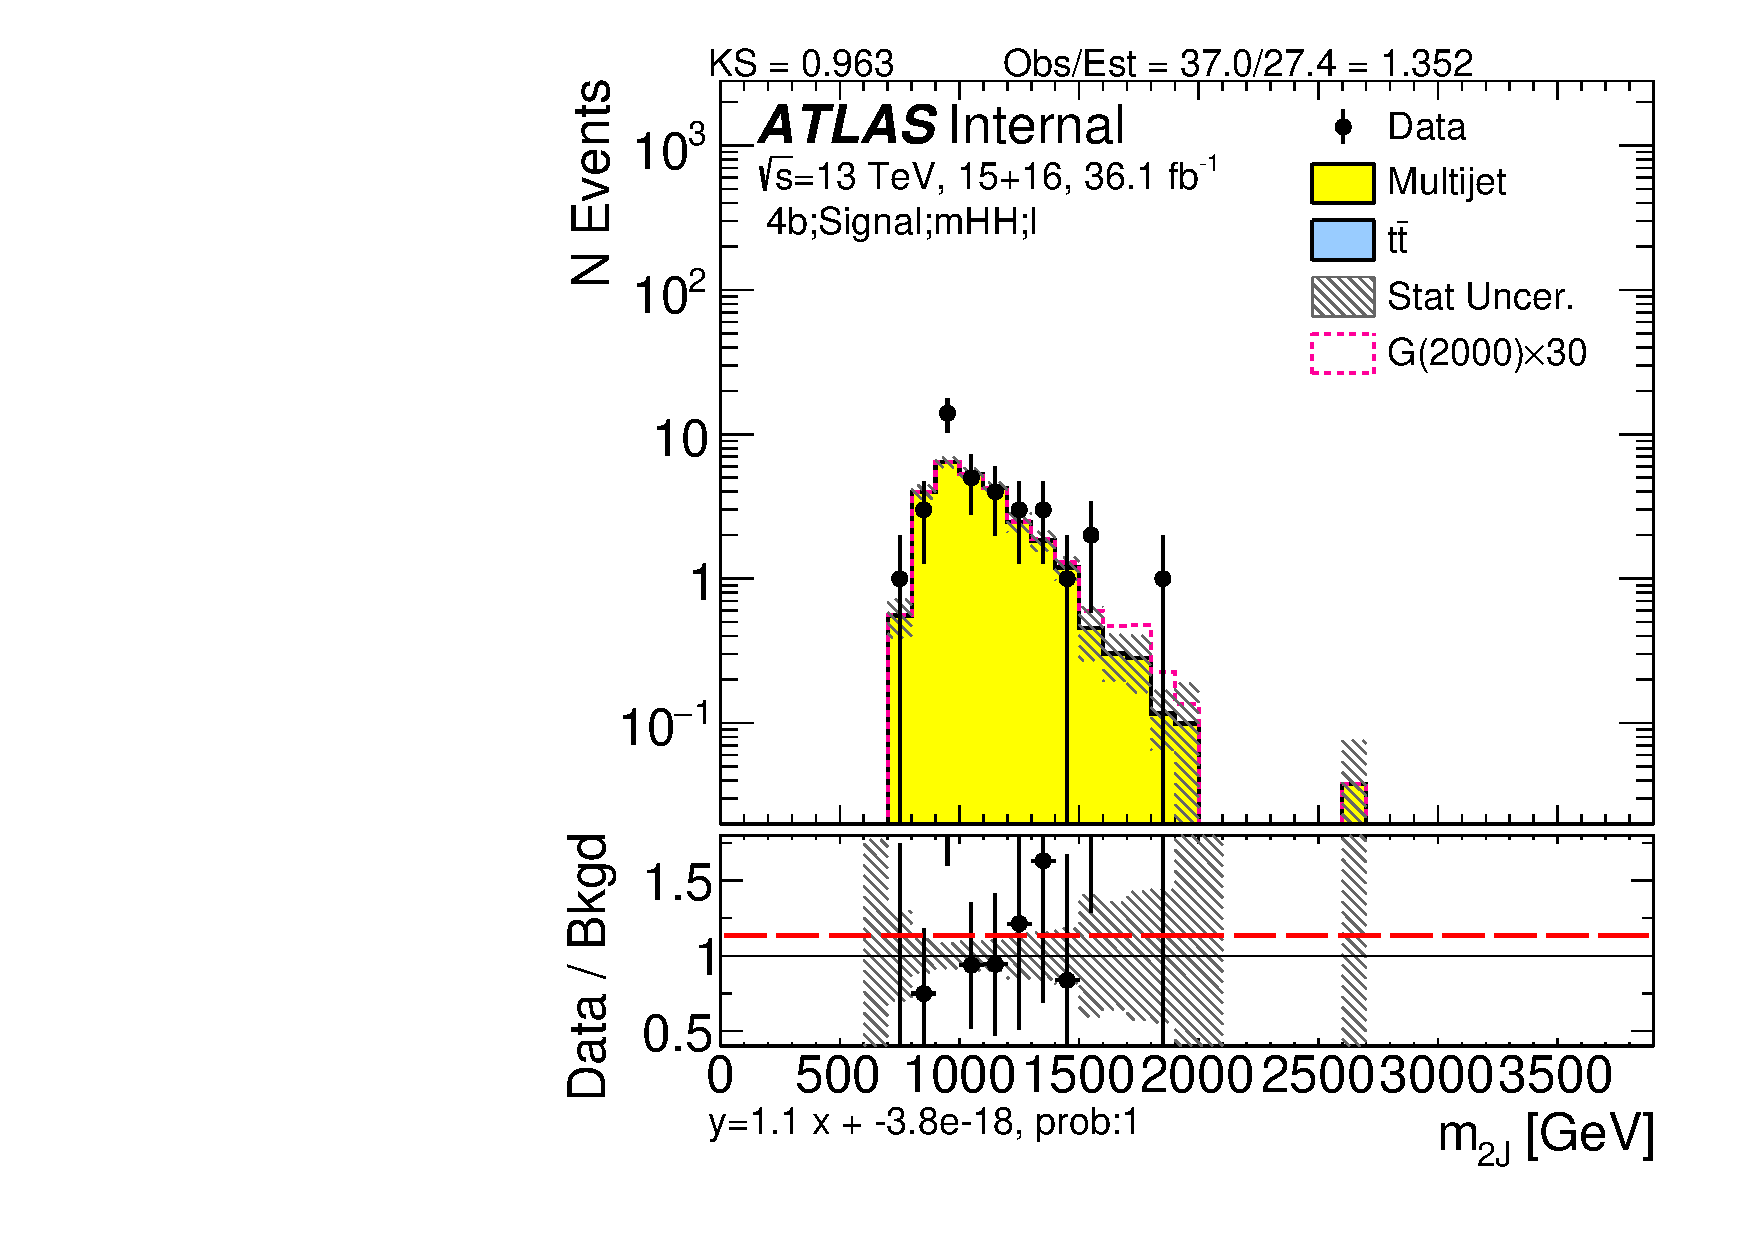
\includegraphics[width=0.41\textwidth,angle=-90]{figures/boosted/ZZ/Moriond_ZZ_FourTag_Signal_mHH_l_1.pdf}
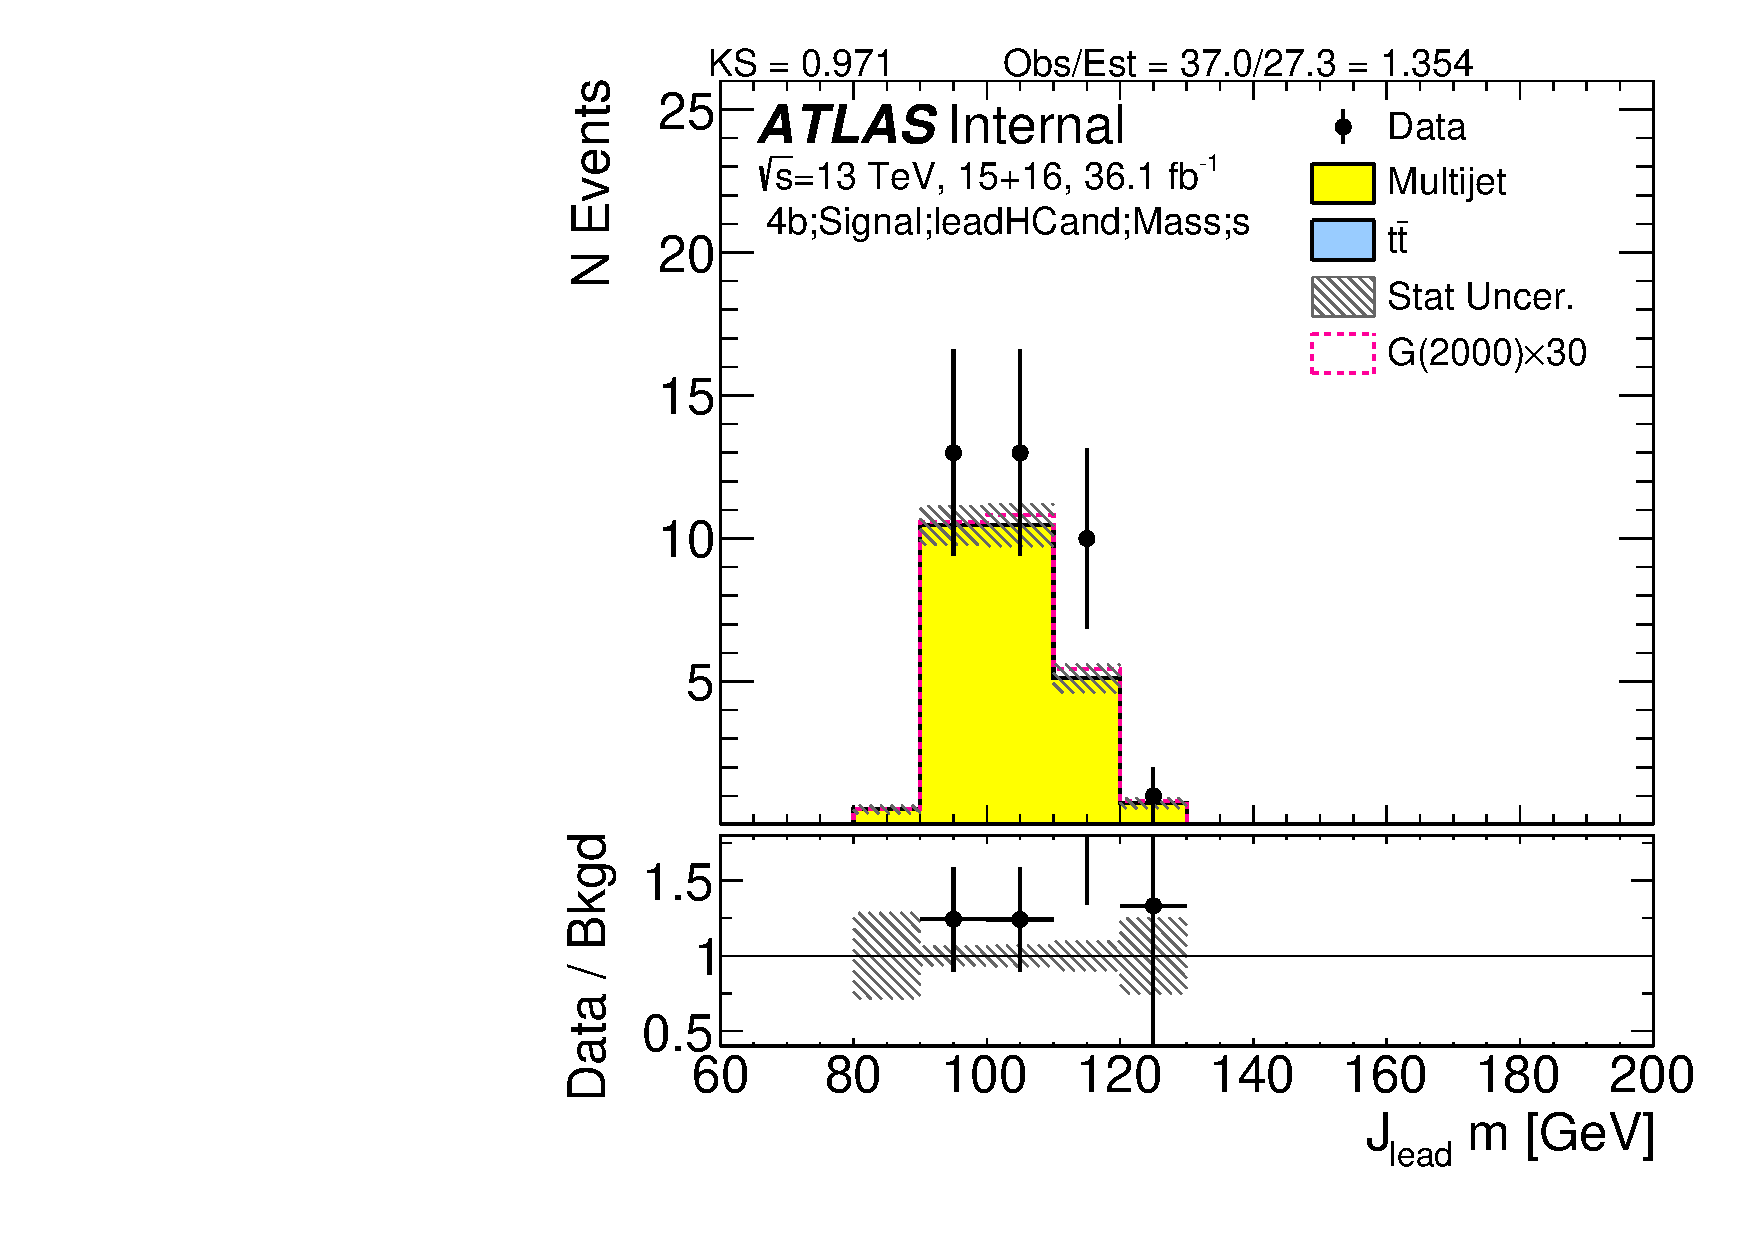
\includegraphics[width=0.41\textwidth,angle=-90]{figures/boosted/ZZ/Moriond_ZZ_FourTag_Signal_leadHCand_Mass_s.pdf}\\
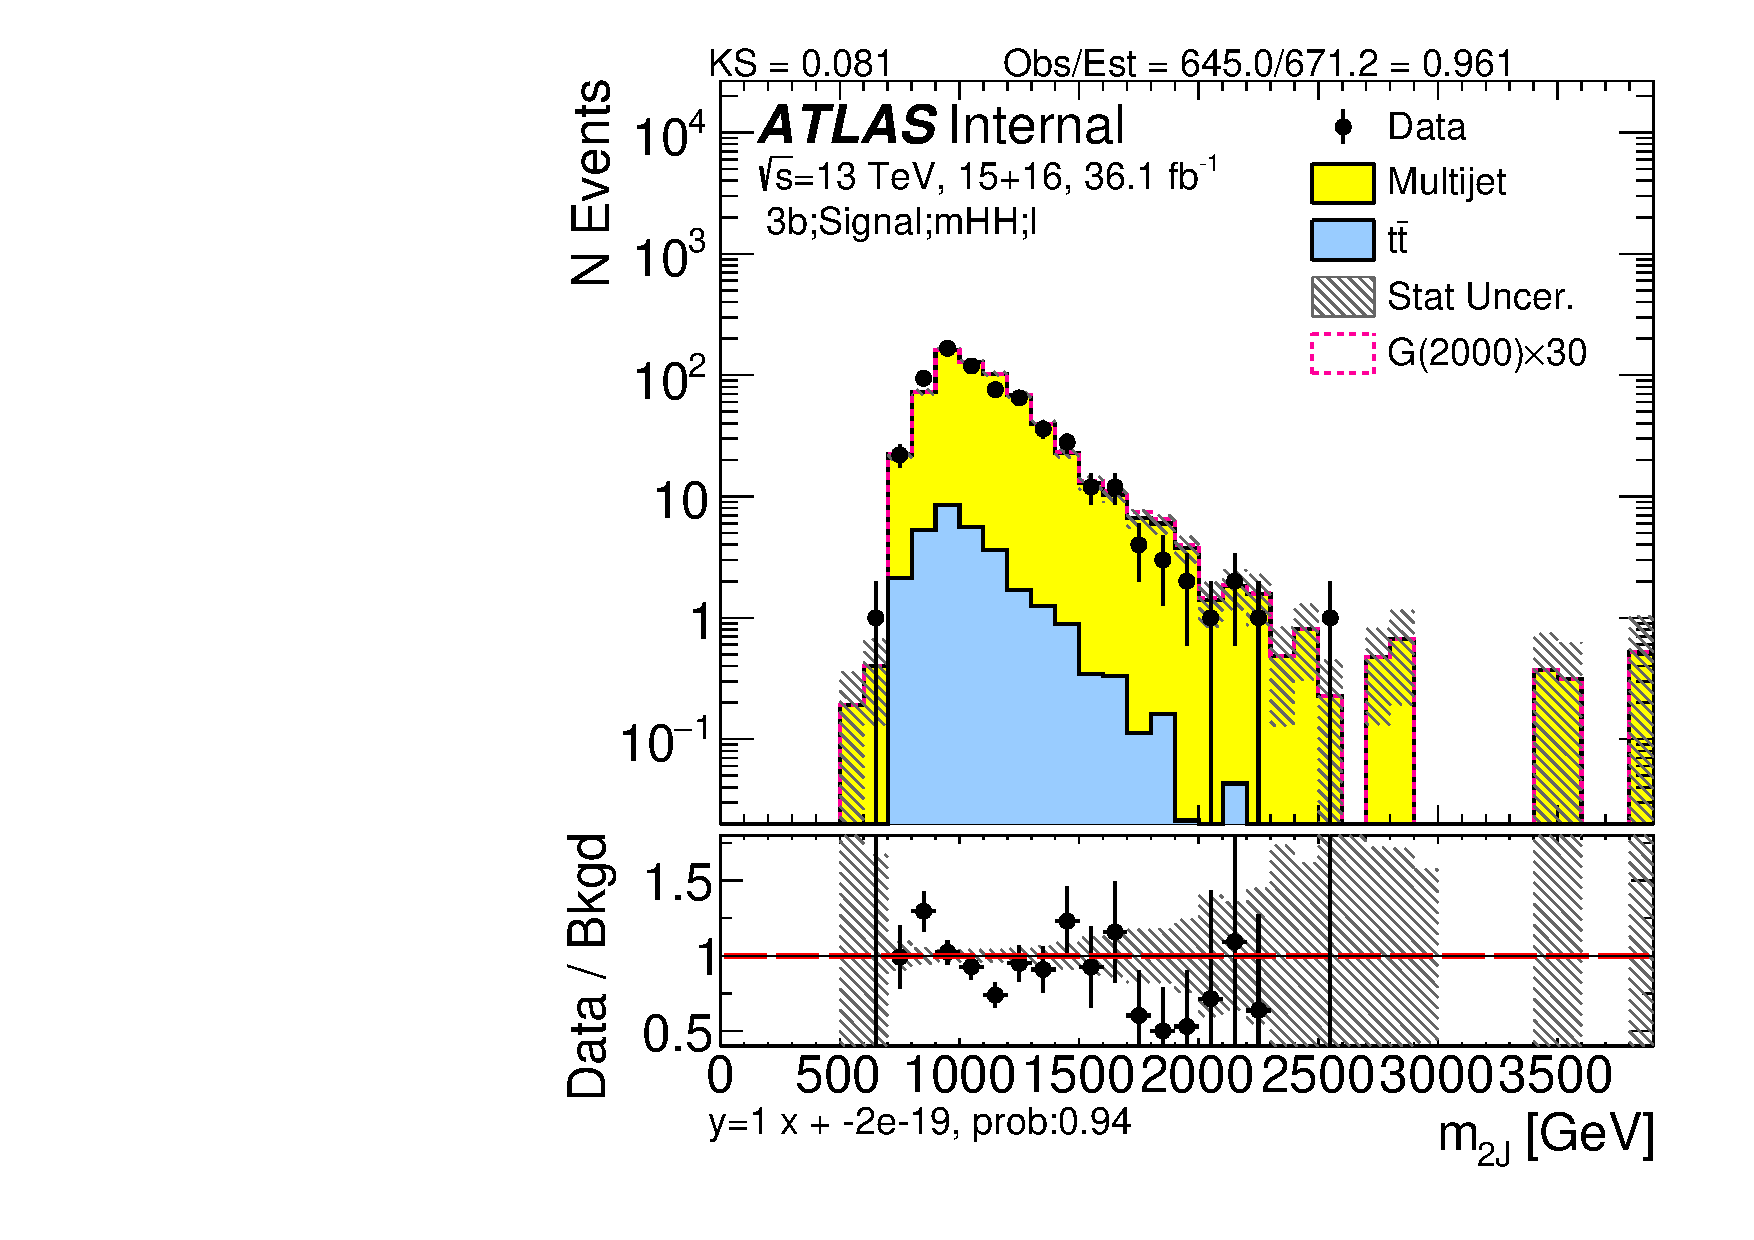
\includegraphics[width=0.41\textwidth,angle=-90]{figures/boosted/ZZ/Moriond_ZZ_ThreeTag_Signal_mHH_l_1.pdf}
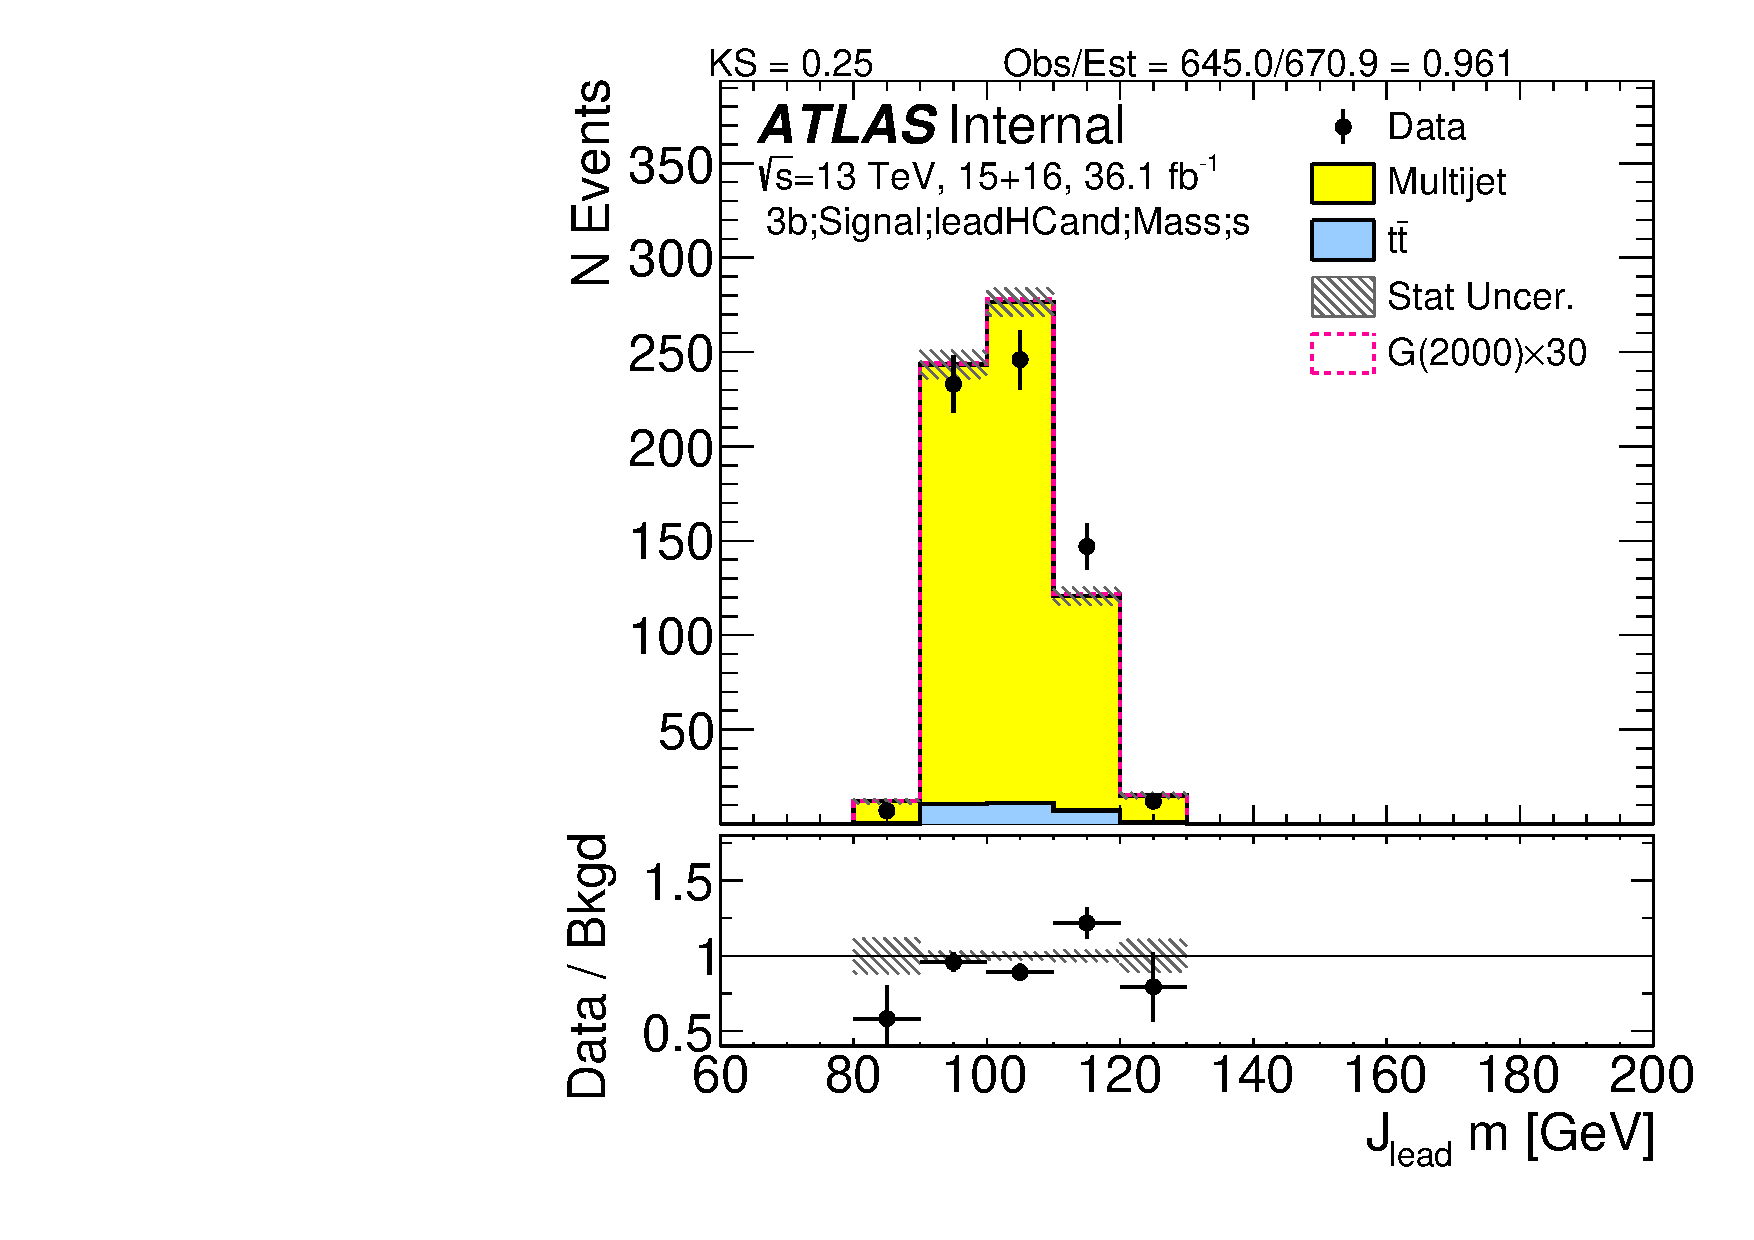
\includegraphics[width=0.41\textwidth,angle=-90]{figures/boosted/ZZ/Moriond_ZZ_ThreeTag_Signal_leadHCand_Mass_s.pdf}\\
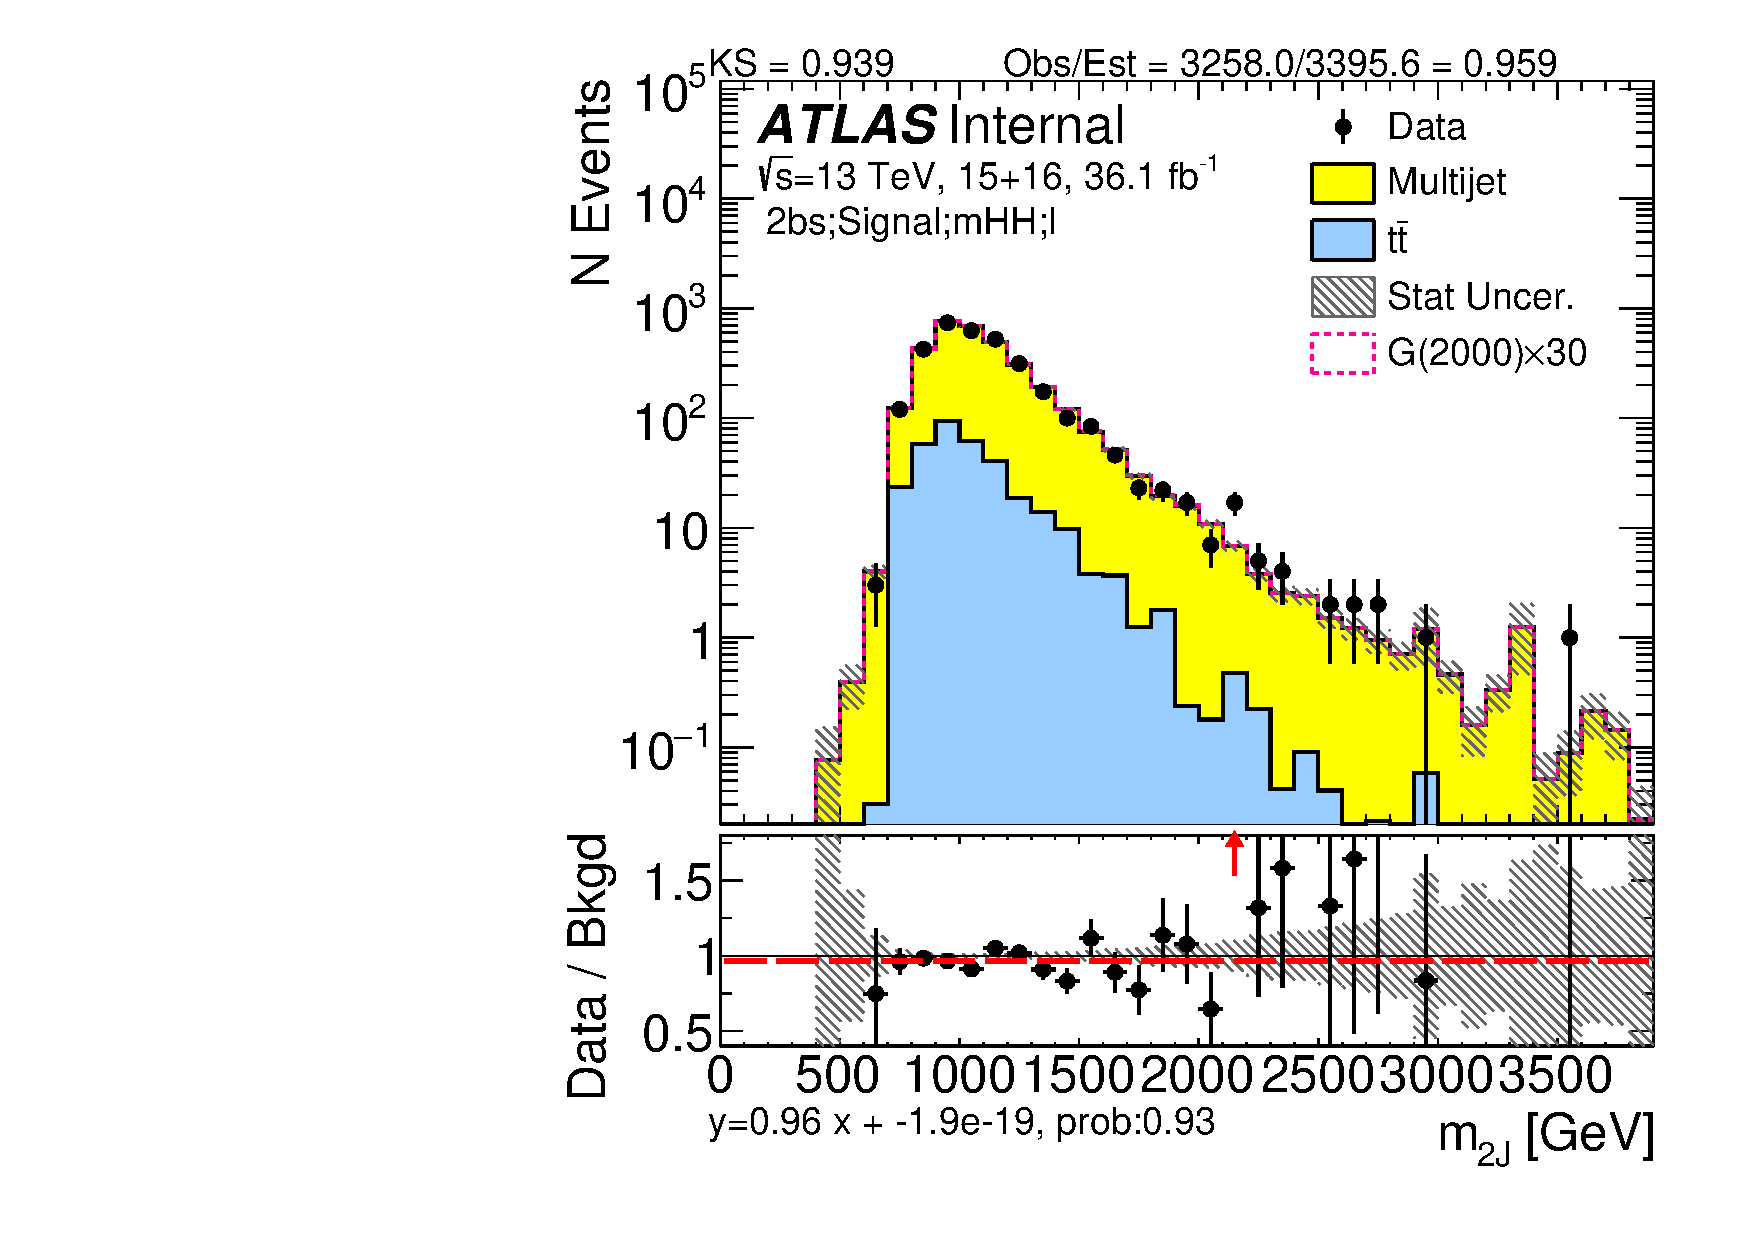
\includegraphics[width=0.41\textwidth,angle=-90]{figures/boosted/ZZ/Moriond_ZZ_TwoTag_split_Signal_mHH_l_1.pdf}
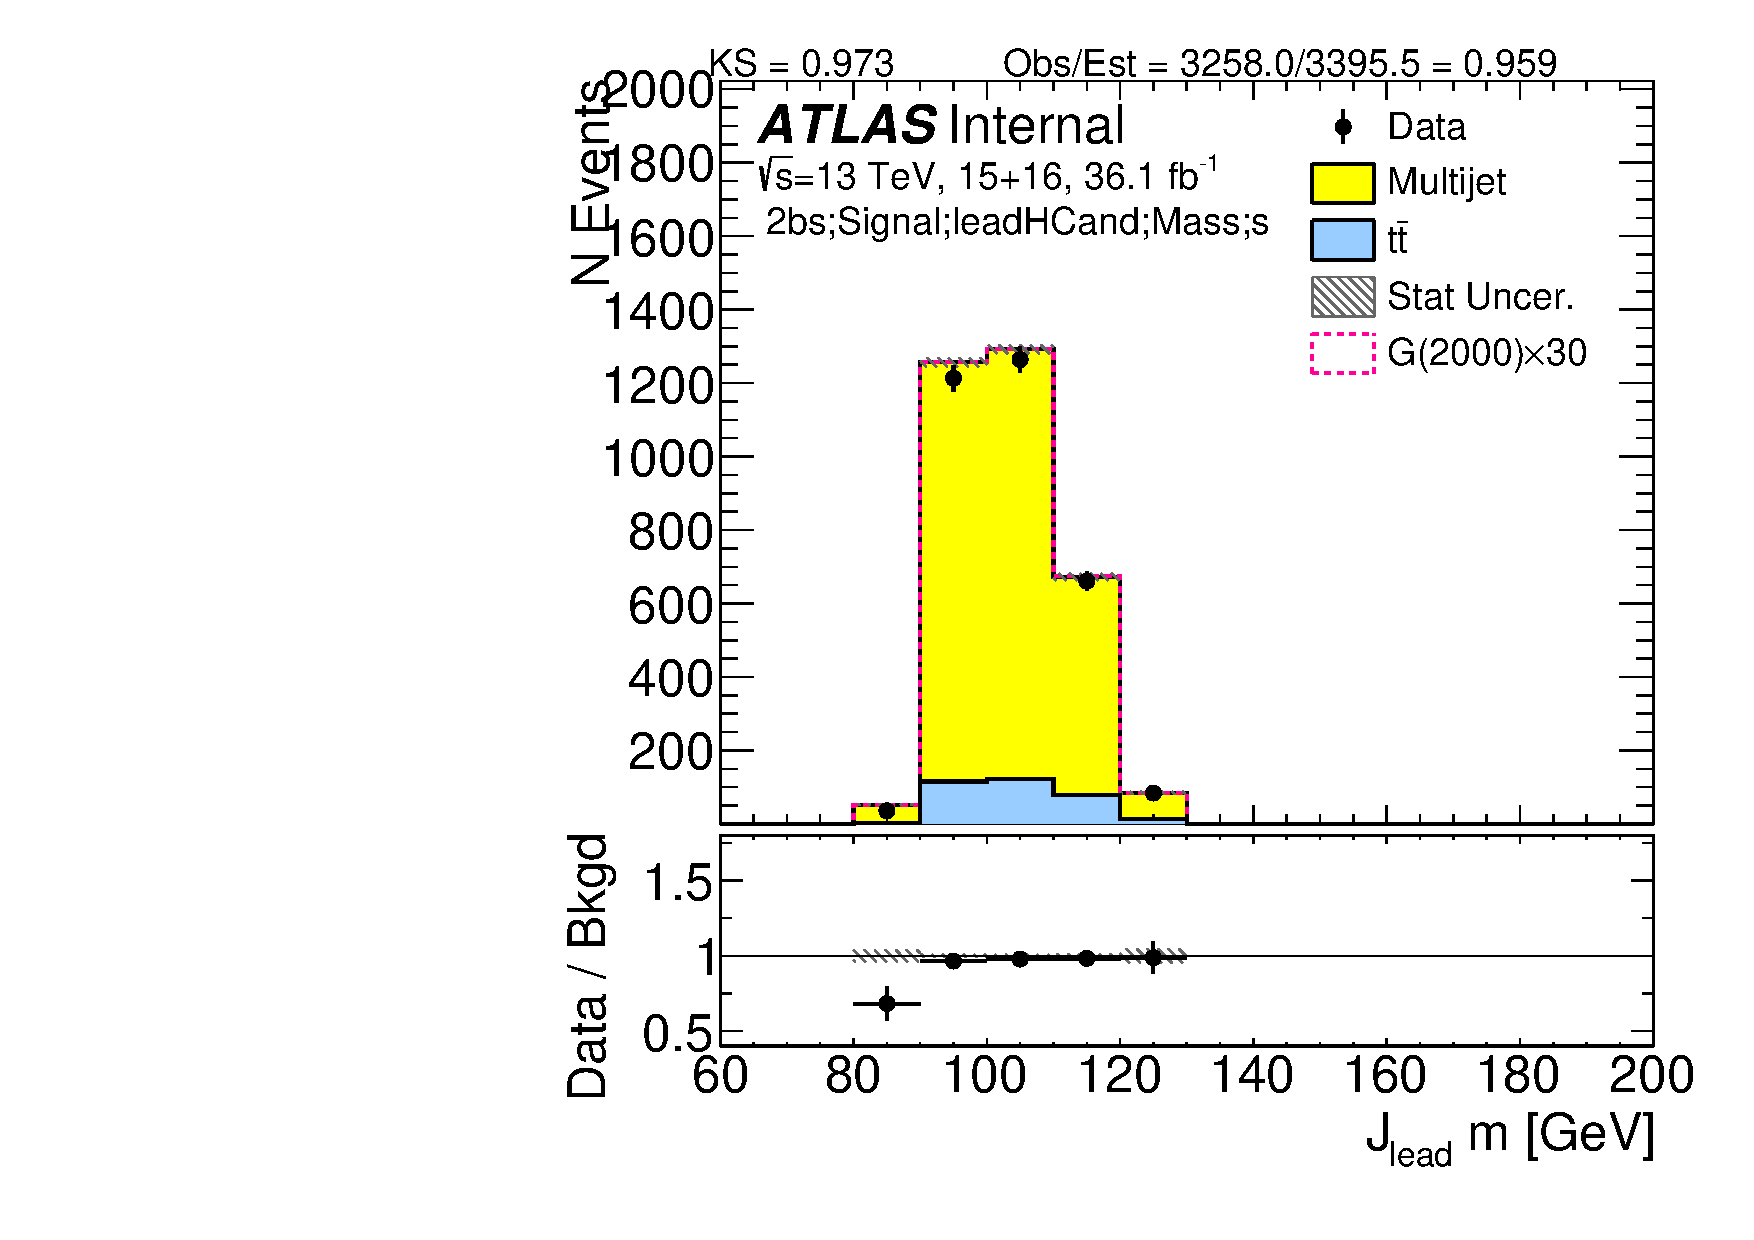
\includegraphics[width=0.41\textwidth,angle=-90]{figures/boosted/ZZ/Moriond_ZZ_TwoTag_split_Signal_leadHCand_Mass_s.pdf}\\
\end{center}
\caption{ZZ signal region distribution of \mtwoJ~ (left column) and leading large-R jet mass (right column), for $4b$ (top row), $3b$ (middle row), and $2bs$ (bottom row). Only statistical uncertainties are shown.}
\label{fig:ZZSR_Distribution}
\end{figure}

% \begin{table}[htb!]
% \begin{center}
% \begin{footnotesize} 
\begin{tabular}{c|c|c|c} 
FourTag & Sideband & Control & Signal \\ 
\hline\hline 
& & & \\ 
QCD Est & 152.28 $\pm$ 2.72 & 63.47 $\pm$ 1.77 & 28.6 $\pm$ 1.21\\ 
$t\bar{t}$ Est.  & 19.86 $\pm$ 0.22 & 7.45 $\pm$ 0.15 & 15.02 $\pm$ 0.2\\ 
$Z+jets$ & 0 $\pm$ 0 & 6.18 $\pm$ 5.12 & 0 $\pm$ 0\\ 
Total Bkg Est & 172.14 $\pm$ 2.73 & 77.1 $\pm$ 5.42 & 43.62 $\pm$ 1.23\\ 
Data & 172.0 $\pm$ 13.11 & 81.0 $\pm$ 9.0 & 46.0 $\pm$ 6.78\\ 
$c=1.0$,$m=1.0TeV$ & 2.38 $\pm$ 0.097 & 5.4 $\pm$ 0.15 & 0.15 $\pm$ 0.024\\ 
$c=1.0$,$m=2.0TeV$ & 0.033 $\pm$ 0.0015 & 0.1 $\pm$ 0.0026 & 0.0011 $\pm$ 0.00027\\ 
$c=1.0$,$m=3.0TeV$ & 0.00031 $\pm$ 3.6e-05 & 0.0008 $\pm$ 5.6e-05 & 1.5e-05 $\pm$ 7.7e-06\\ 
& & & \\ 
\hline\hline 
\end{tabular} 
\end{footnotesize} 
\newline 

% \end{center}
% \caption{Background prediction in SR/CR/SB for TT SR in $4b$-tag region. Uncertainties are stat only.}
% \label{CRSB:SummaryTable_TT_4b}
% \end{table}

% \begin{table}[htb!]
% \begin{center}
% \begin{footnotesize} 
\begin{tabular}{c|c|c|c} 
ThreeTag & Sideband & Control & Signal \\ 
\hline\hline 
QCD Est & 3106.11 $\pm$ 25.79 & 1427.41 $\pm$ 17.53 & 570.01 $\pm$ 11.6\\ 
$t\bar{t}$ Est.  & 495.21 $\pm$ 18.75 & 148.55 $\pm$ 10.21 & 406.57 $\pm$ 5.42\\ 
$Z+jets$ & 32.5 $\pm$ 11.34 & 11.21 $\pm$ 5.65 & 0.3 $\pm$ 0.3\\ 
Total Bkg Est & 3633.82 $\pm$ 33.85 & 1587.17 $\pm$ 21.05 & 976.88 $\pm$ 12.81\\ 
Data & 3633.0 $\pm$ 60.27 & 1553.0 $\pm$ 39.41 & 1017.0 $\pm$ 31.89\\ 
$c=1.0$,$m=1.0TeV$ & 7.57 $\pm$ 0.18 & 12.58 $\pm$ 0.23 & 0.32 $\pm$ 0.037\\ 
$c=1.0$,$m=2.0TeV$ & 0.15 $\pm$ 0.0034 & 0.38 $\pm$ 0.0054 & 0.0047 $\pm$ 0.0006\\ 
$c=1.0$,$m=3.0TeV$ & 0.0034 $\pm$ 0.00012 & 0.0075 $\pm$ 0.00018 & 0.00023 $\pm$ 3.3e-05\\ 
\hline\hline 
\end{tabular} 
\end{footnotesize} 
\newline 

% \end{center}
% \caption{Background prediction in SR/CR/SB for TT SR in $3b$-tag region. Uncertainties are stat only.}
% \label{CRSB:SummaryTable_TT_3b}
% \end{table}

% \begin{table}[htb!]
% \begin{center}
% \begin{footnotesize} 
\begin{tabular}{c|c|c|c} 
TwoTag split & Sideband & Control & Signal \\ 
\hline\hline 
QCD Est & 14980.05 $\pm$ 35.33 & 6803.06 $\pm$ 23.41 & 2817.92 $\pm$ 16.54\\ 
$t\bar{t}$ Est.  & 5170.92 $\pm$ 56.22 & 1468.85 $\pm$ 28.93 & 3628.91 $\pm$ 48.42\\ 
$Z+jets$ & 61.34 $\pm$ 16.04 & 26.44 $\pm$ 10.08 & 6.4 $\pm$ 5.05\\ 
Total Bkg Est & 20212.31 $\pm$ 68.31 & 8298.34 $\pm$ 38.56 & 6453.23 $\pm$ 51.41\\ 
Data & 20212.0 $\pm$ 142.17 & 8486.0 $\pm$ 92.12 & 6446.0 $\pm$ 80.29\\ 
$c=1.0$,$m=1.0TeV$ & 4.59 $\pm$ 0.14 & 6.33 $\pm$ 0.16 & 0.24 $\pm$ 0.033\\ 
$c=1.0$,$m=2.0TeV$ & 0.17 $\pm$ 0.0039 & 0.36 $\pm$ 0.0056 & 0.0066 $\pm$ 0.00077\\ 
$c=1.0$,$m=3.0TeV$ & 0.012 $\pm$ 0.00024 & 0.027 $\pm$ 0.00034 & 0.00089 $\pm$ 6.7e-05\\ 
\hline\hline 
\end{tabular} 
\end{footnotesize} 
\newline 

% \end{center}
% \caption{Background prediction in SR/CR/SB for TT SR in $2bs$-tag region. Uncertainties are stat only.}
% \label{CRSB:SummaryTable_TT_2b}
% \end{table}


\begin{figure}[htb!]
\begin{center}
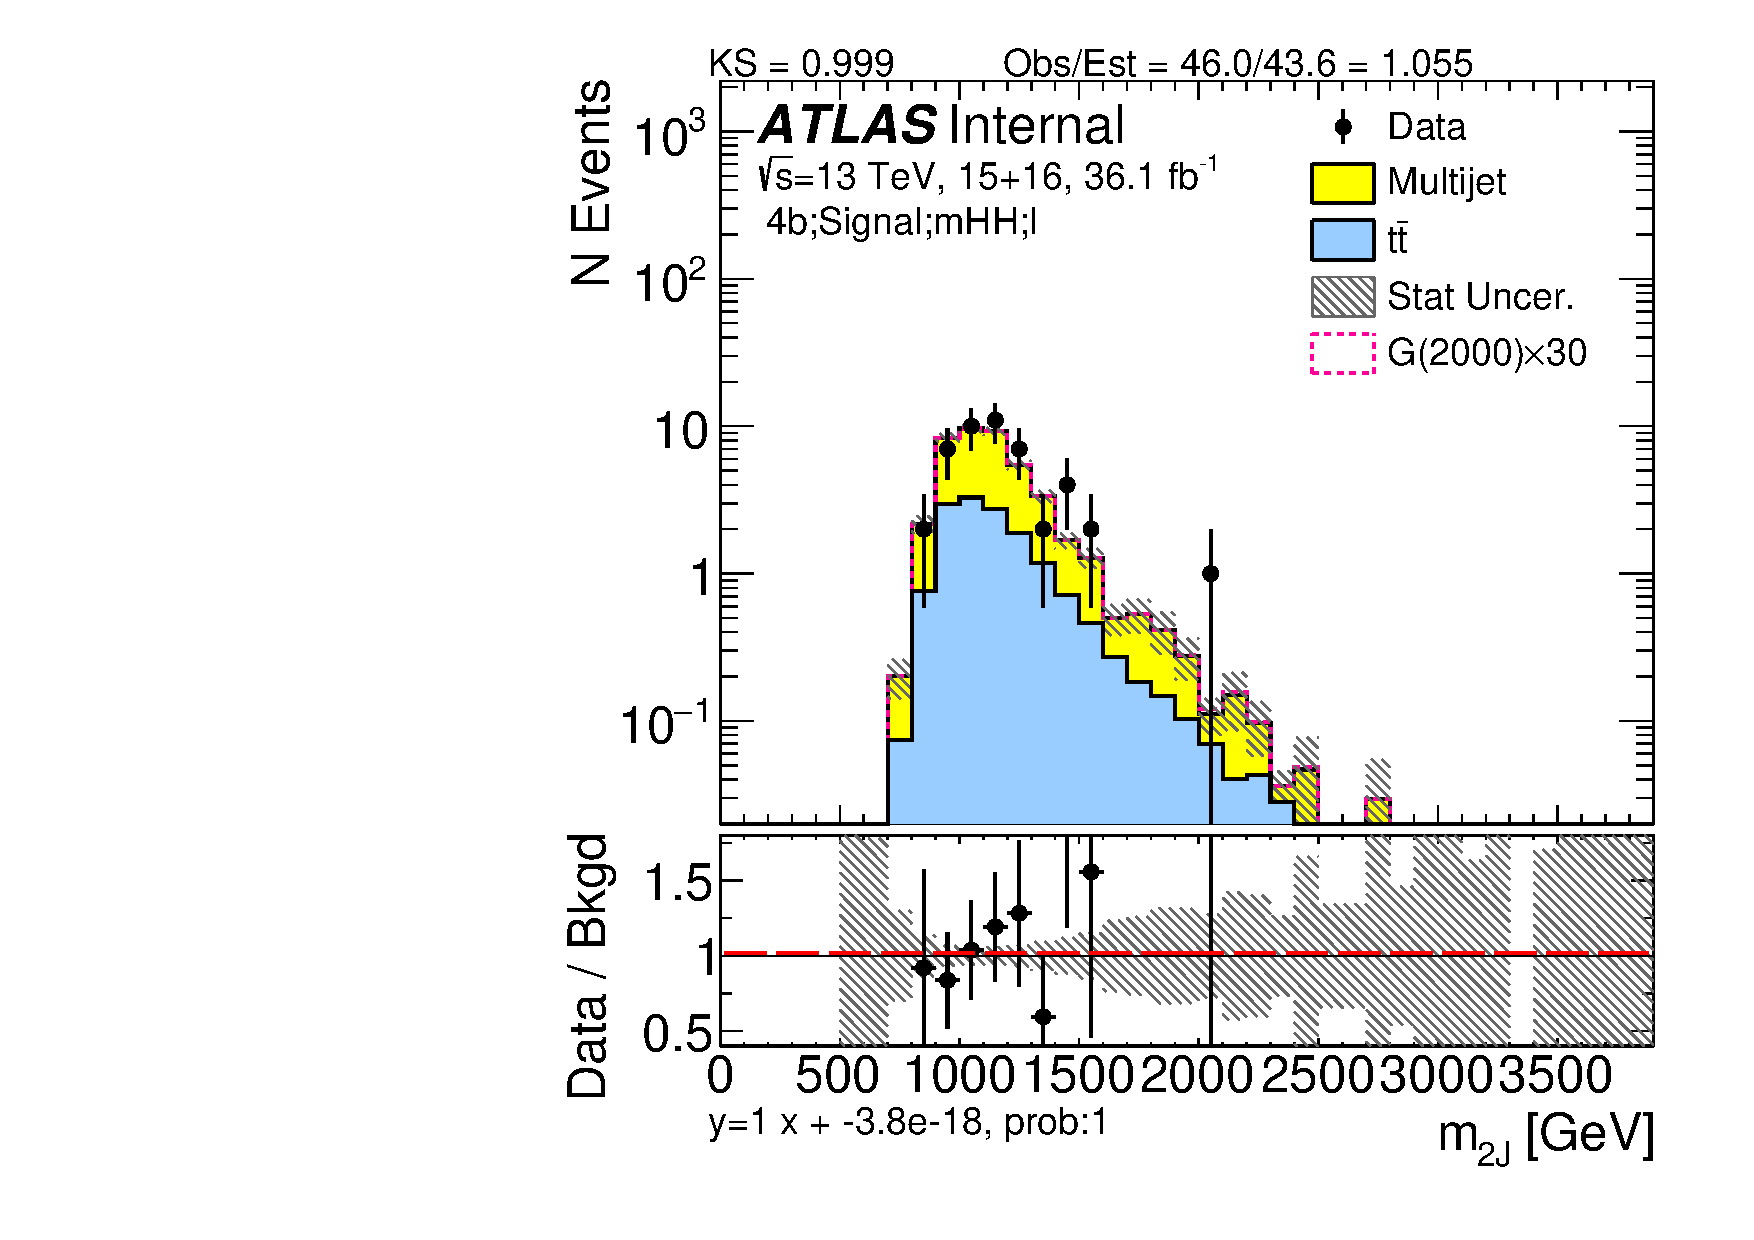
\includegraphics[width=0.41\textwidth,angle=-90]{figures/boosted/TT/Moriond_TT_FourTag_Signal_mHH_l_1.pdf}
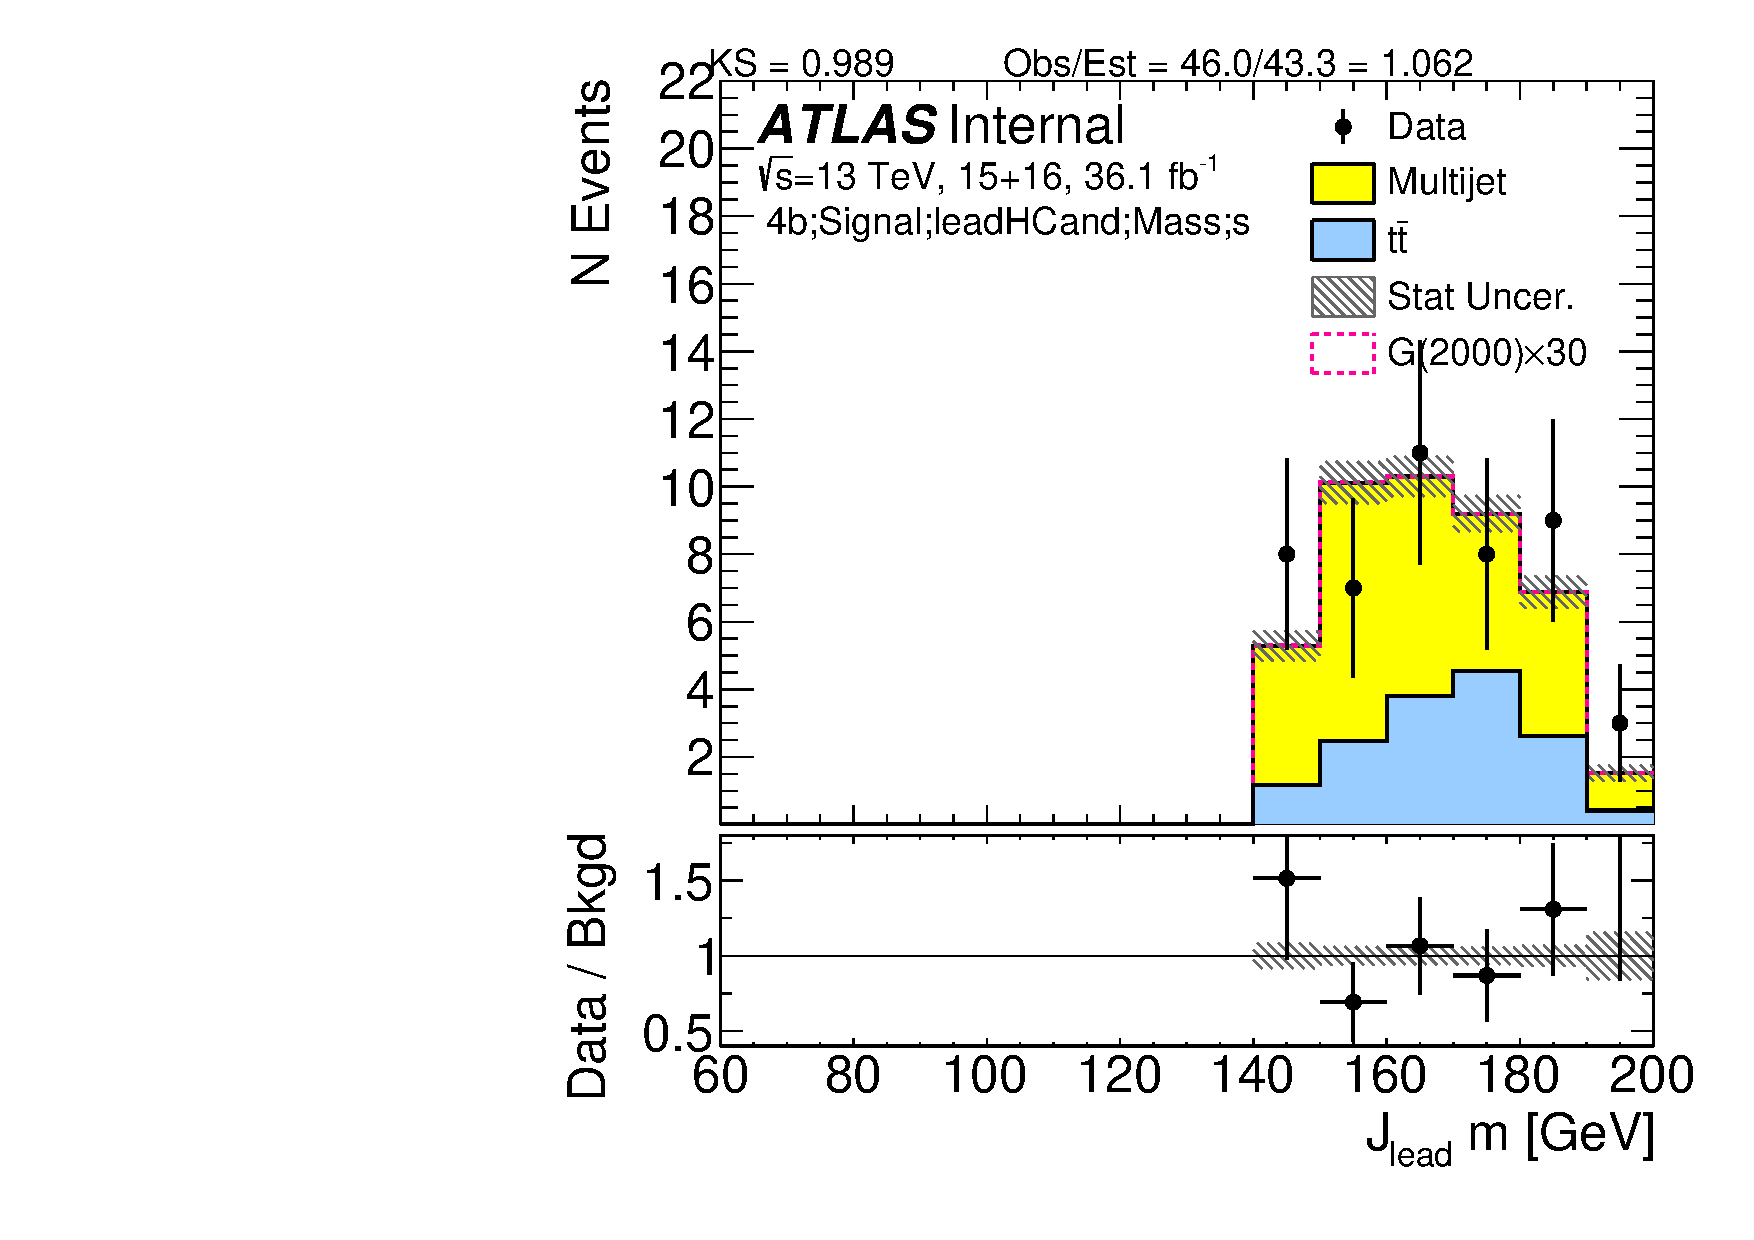
\includegraphics[width=0.41\textwidth,angle=-90]{figures/boosted/TT/Moriond_TT_FourTag_Signal_leadHCand_Mass_s.pdf}\\
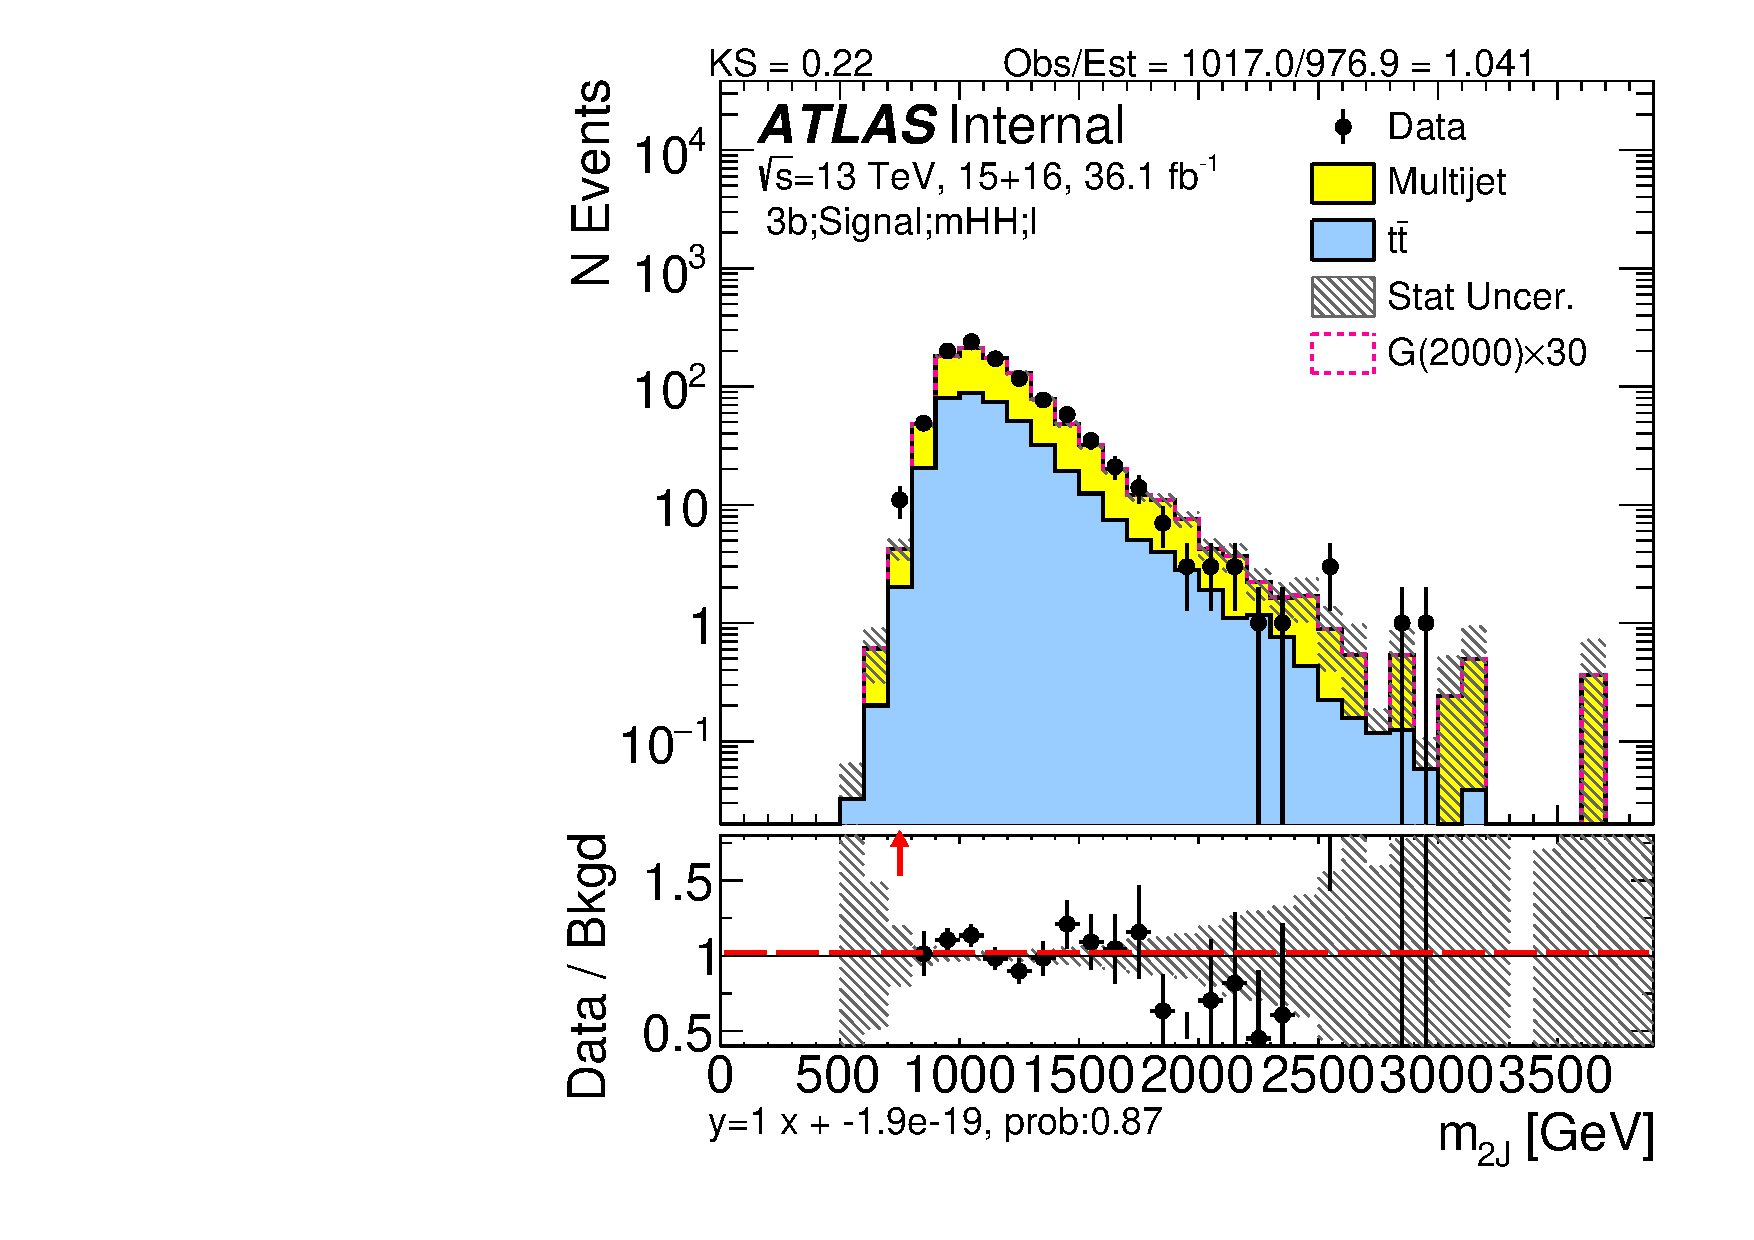
\includegraphics[width=0.41\textwidth,angle=-90]{figures/boosted/TT/Moriond_TT_ThreeTag_Signal_mHH_l_1.pdf}
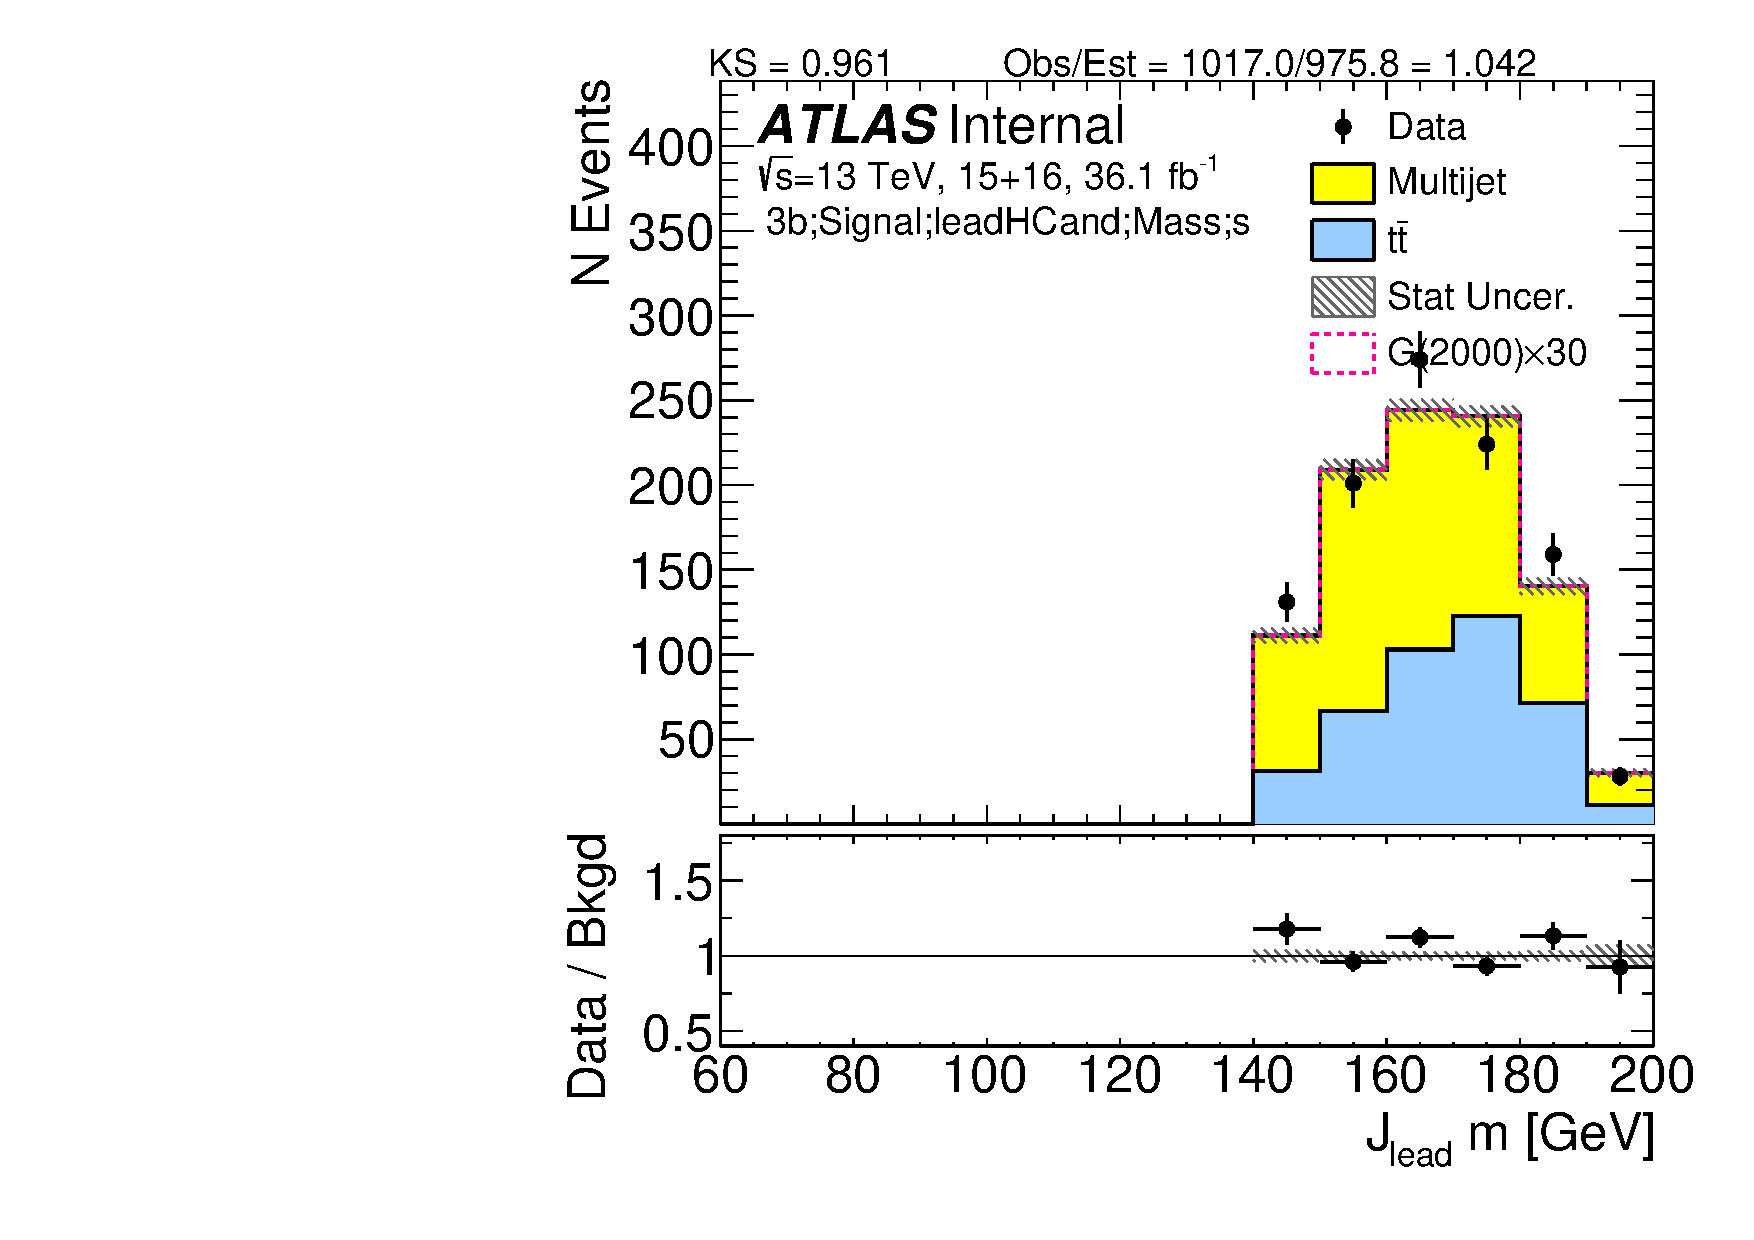
\includegraphics[width=0.41\textwidth,angle=-90]{figures/boosted/TT/Moriond_TT_ThreeTag_Signal_leadHCand_Mass_s.pdf}\\
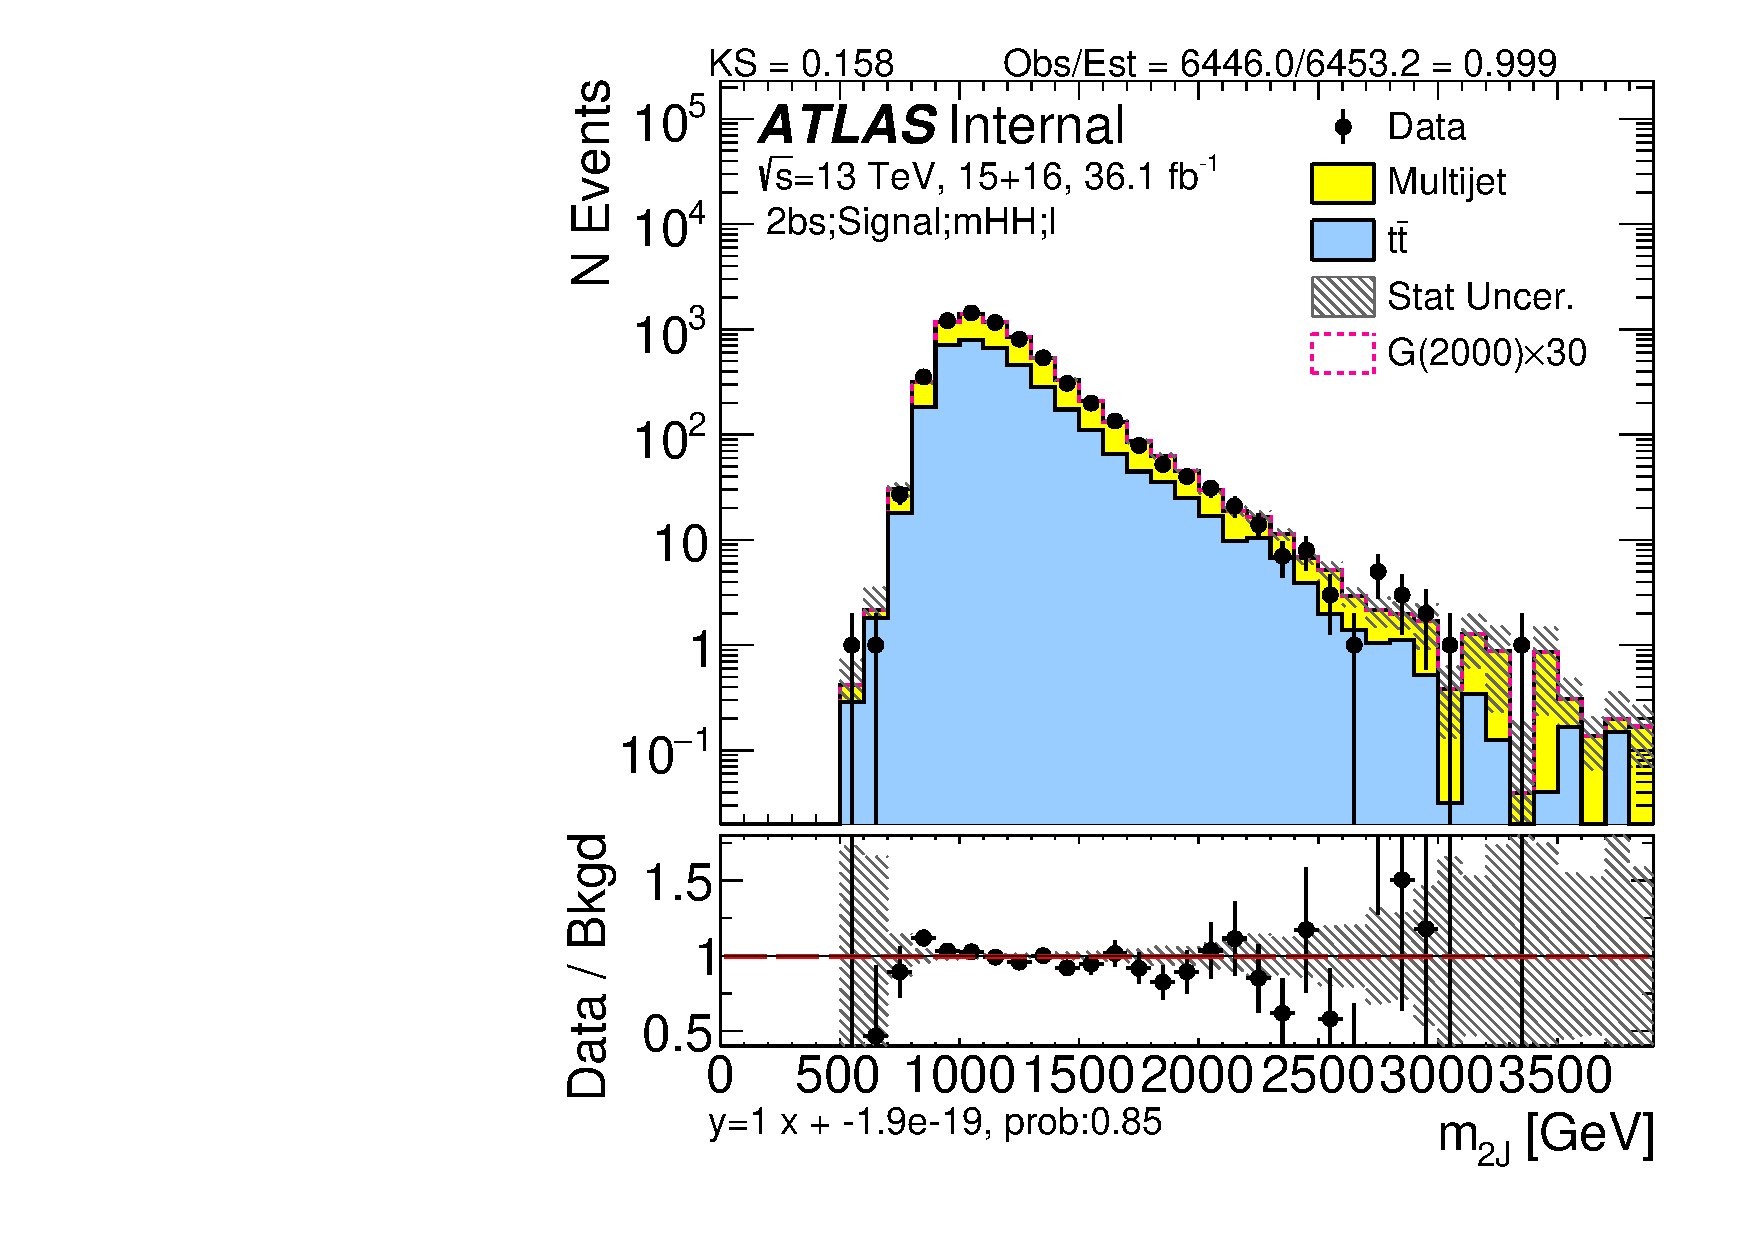
\includegraphics[width=0.41\textwidth,angle=-90]{figures/boosted/TT/Moriond_TT_TwoTag_split_Signal_mHH_l_1.pdf}
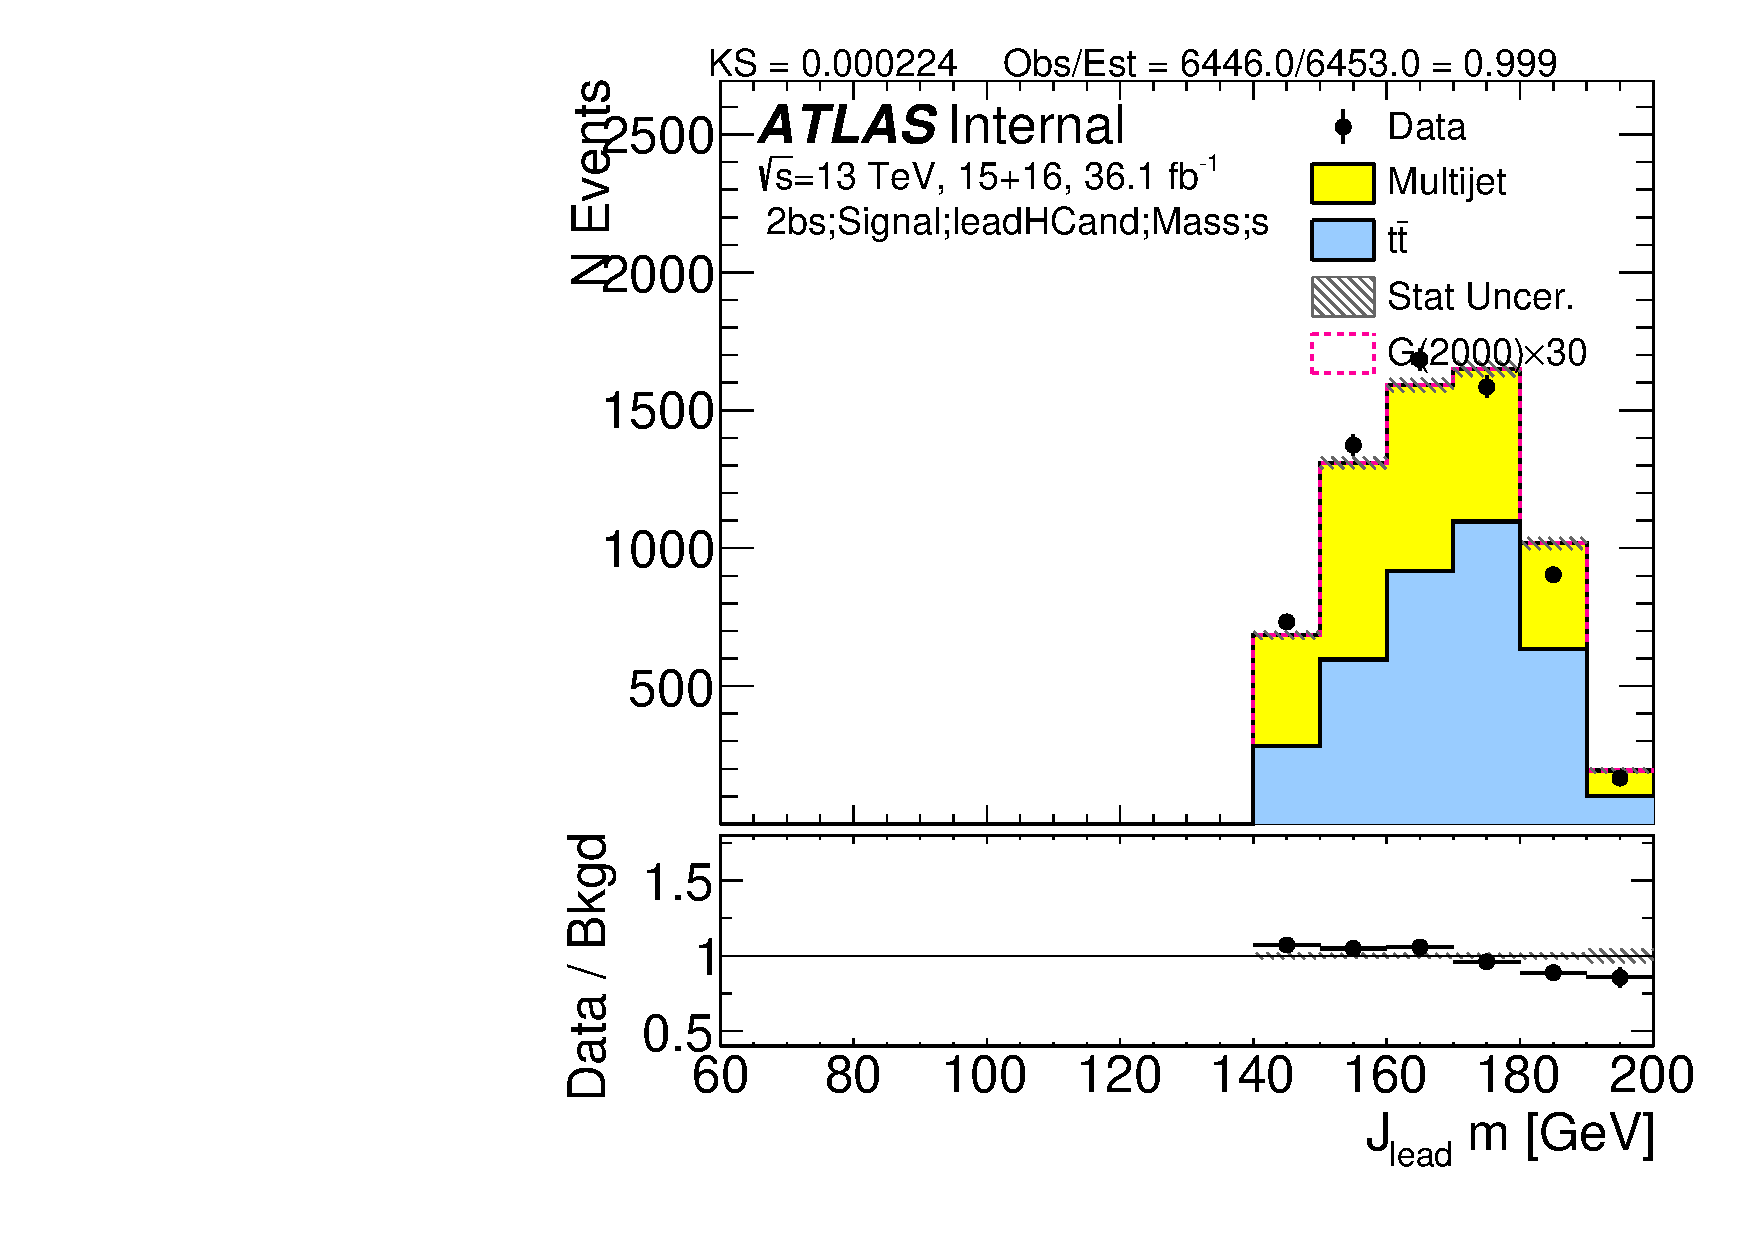
\includegraphics[width=0.41\textwidth,angle=-90]{figures/boosted/TT/Moriond_TT_TwoTag_split_Signal_leadHCand_Mass_s.pdf}\\
\end{center}
\caption{TT signal region distribution of \mtwoJ~ (left column) and leading large-R jet mass (right column), for $4b$ (top row), $3b$ (middle row), and $2bs$ (bottom row). Only statistical uncertainties are shown.}
\label{fig:TTSR_Distribution}
\end{figure}
